The manuscript now reports leakage-free forecasting results, uncertainty-calibration checks, cross-entity transfer checks, broad service-level evidence from official container traces, and a calibrated control comparison based on a trainable uncertainty-aware surrogate. The evidence is strong enough for a multi-granularity discussion, while still leaving room for service-aware tuning and stronger deep temporal models.

\subsection{Forecasting benchmark}

The experimental pipeline includes a reproducible downloader for Alibaba \texttt{v2018} artifacts, a preprocessing route that builds a one-minute aggregate workload series from the compressed trace, baseline forecasters, a trainable \texttt{UA-MSTCN-Lite} surrogate, and a predictive-versus-reactive policy simulator. Most importantly, the reported metrics are computed on 11{,}208 aggregate samples rather than on placeholder values.

Table~\ref{tab:forecast-smoke-test} summarizes aggregate forecasting results under the leakage-free split. Linear regression provides the best average MAE across the three horizons (3.514), random forest is a close second (3.529), and \texttt{UA-MSTCN-Lite} remains competitive rather than dominant (3.548 average MAE). The standard neural MLP baseline improves over persistence and moving average, but its average MAE of 3.708 does not overturn the linear-tree ranking. At the 10-minute horizon, the gap between linear regression and \texttt{UA-MSTCN-Lite} is only 0.0013 MAE, which is small enough to treat the two models as practically tied on this aggregate signal. The aggregate benchmark therefore shows that the uncertainty-aware surrogate can still support the control study even when it is not the strongest point forecaster.

\begin{table}[htbp]
  \centering
  \caption{Verified smoke-test forecasting performance on the aggregate cluster series.}
  \label{tab:forecast-smoke-test}
  \scriptsize
  \setlength{\tabcolsep}{2pt}
  \renewcommand{\arraystretch}{0.96}
  \begin{tabular}{lcccc}
    \toprule
    Model & Horizon & MAE & RMSE & MAPE \\
    \midrule
    Persistence & 1 & 2.395 & 3.285 & 0.060 \\
    Moving average & 1 & 3.215 & 4.348 & 0.079 \\
    Linear regression & 1 & 2.268 & 3.123 & 0.056 \\
    Random forest & 1 & 2.324 & 3.176 & 0.058 \\
    MLP regressor & 1 & 2.422 & 3.267 & 0.061 \\
    UA-MSTCN-Lite & 1 & 2.349 & 3.214 & 0.058 \\
    Persistence & 5 & 4.569 & 6.162 & 0.112 \\
    Moving average & 5 & 4.387 & 5.850 & 0.107 \\
    Linear regression & 5 & 3.967 & 5.324 & 0.098 \\
    Random forest & 5 & 3.928 & 5.237 & 0.097 \\
    MLP regressor & 5 & 4.276 & 5.603 & 0.105 \\
    UA-MSTCN-Lite & 5 & 3.986 & 5.304 & 0.098 \\
    Persistence & 10 & 5.119 & 6.785 & 0.126 \\
    Moving average & 10 & 4.845 & 6.409 & 0.119 \\
    Linear regression & 10 & 4.307 & 5.765 & 0.107 \\
    Random forest & 10 & 4.334 & 5.780 & 0.107 \\
    MLP regressor & 10 & 4.427 & 5.781 & 0.109 \\
    UA-MSTCN-Lite & 10 & 4.308 & 5.793 & 0.107 \\
    \bottomrule
  \end{tabular}
\end{table}

\begin{figure}[htbp]
  \centering
  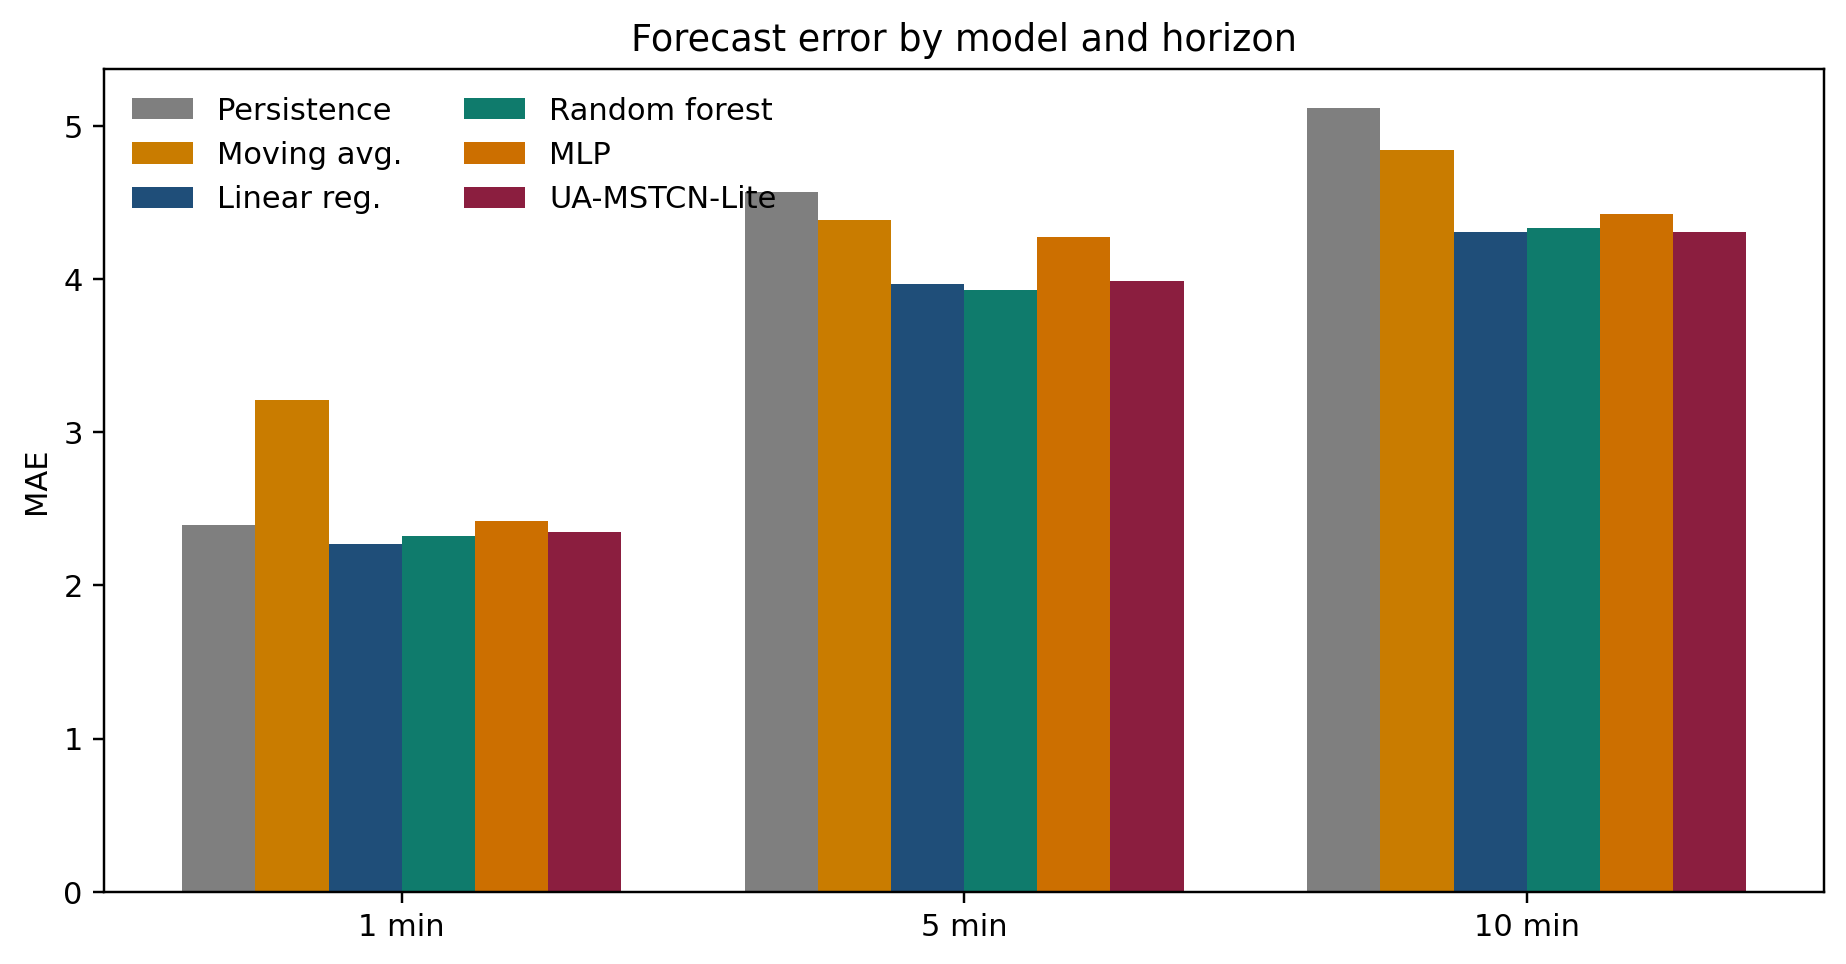
\includegraphics[width=\linewidth]{../experiments/results/figures/baseline_mae_by_horizon.png}
  \caption{Forecast error by model and horizon after the leakage-free split correction. Linear regression remains the strongest average point forecaster, while the standard neural MLP baseline improves over simple heuristics without changing the overall ranking.}
  \label{fig:mae-by-horizon}
\end{figure}

\subsection{Case study and accuracy-runtime trade-off}

Aggregate error tables alone do not show where the models succeed or fail. Figure~\ref{fig:forecast-case-study} therefore plots aligned slices from the test set at the 1-, 5-, and 10-minute horizons. The same pattern appears across horizons: persistence reacts too slowly when the workload turns, the MLP captures the broad trend but remains smoother around turning points, and random forest together with \texttt{UA-MSTCN-Lite} tracks the main shape more closely. The figure is still useful even though \texttt{UA-MSTCN-Lite} is no longer the best average point forecaster, because the controller consumes its quantile band rather than only its median prediction.

\begin{figure}[htbp]
  \centering
  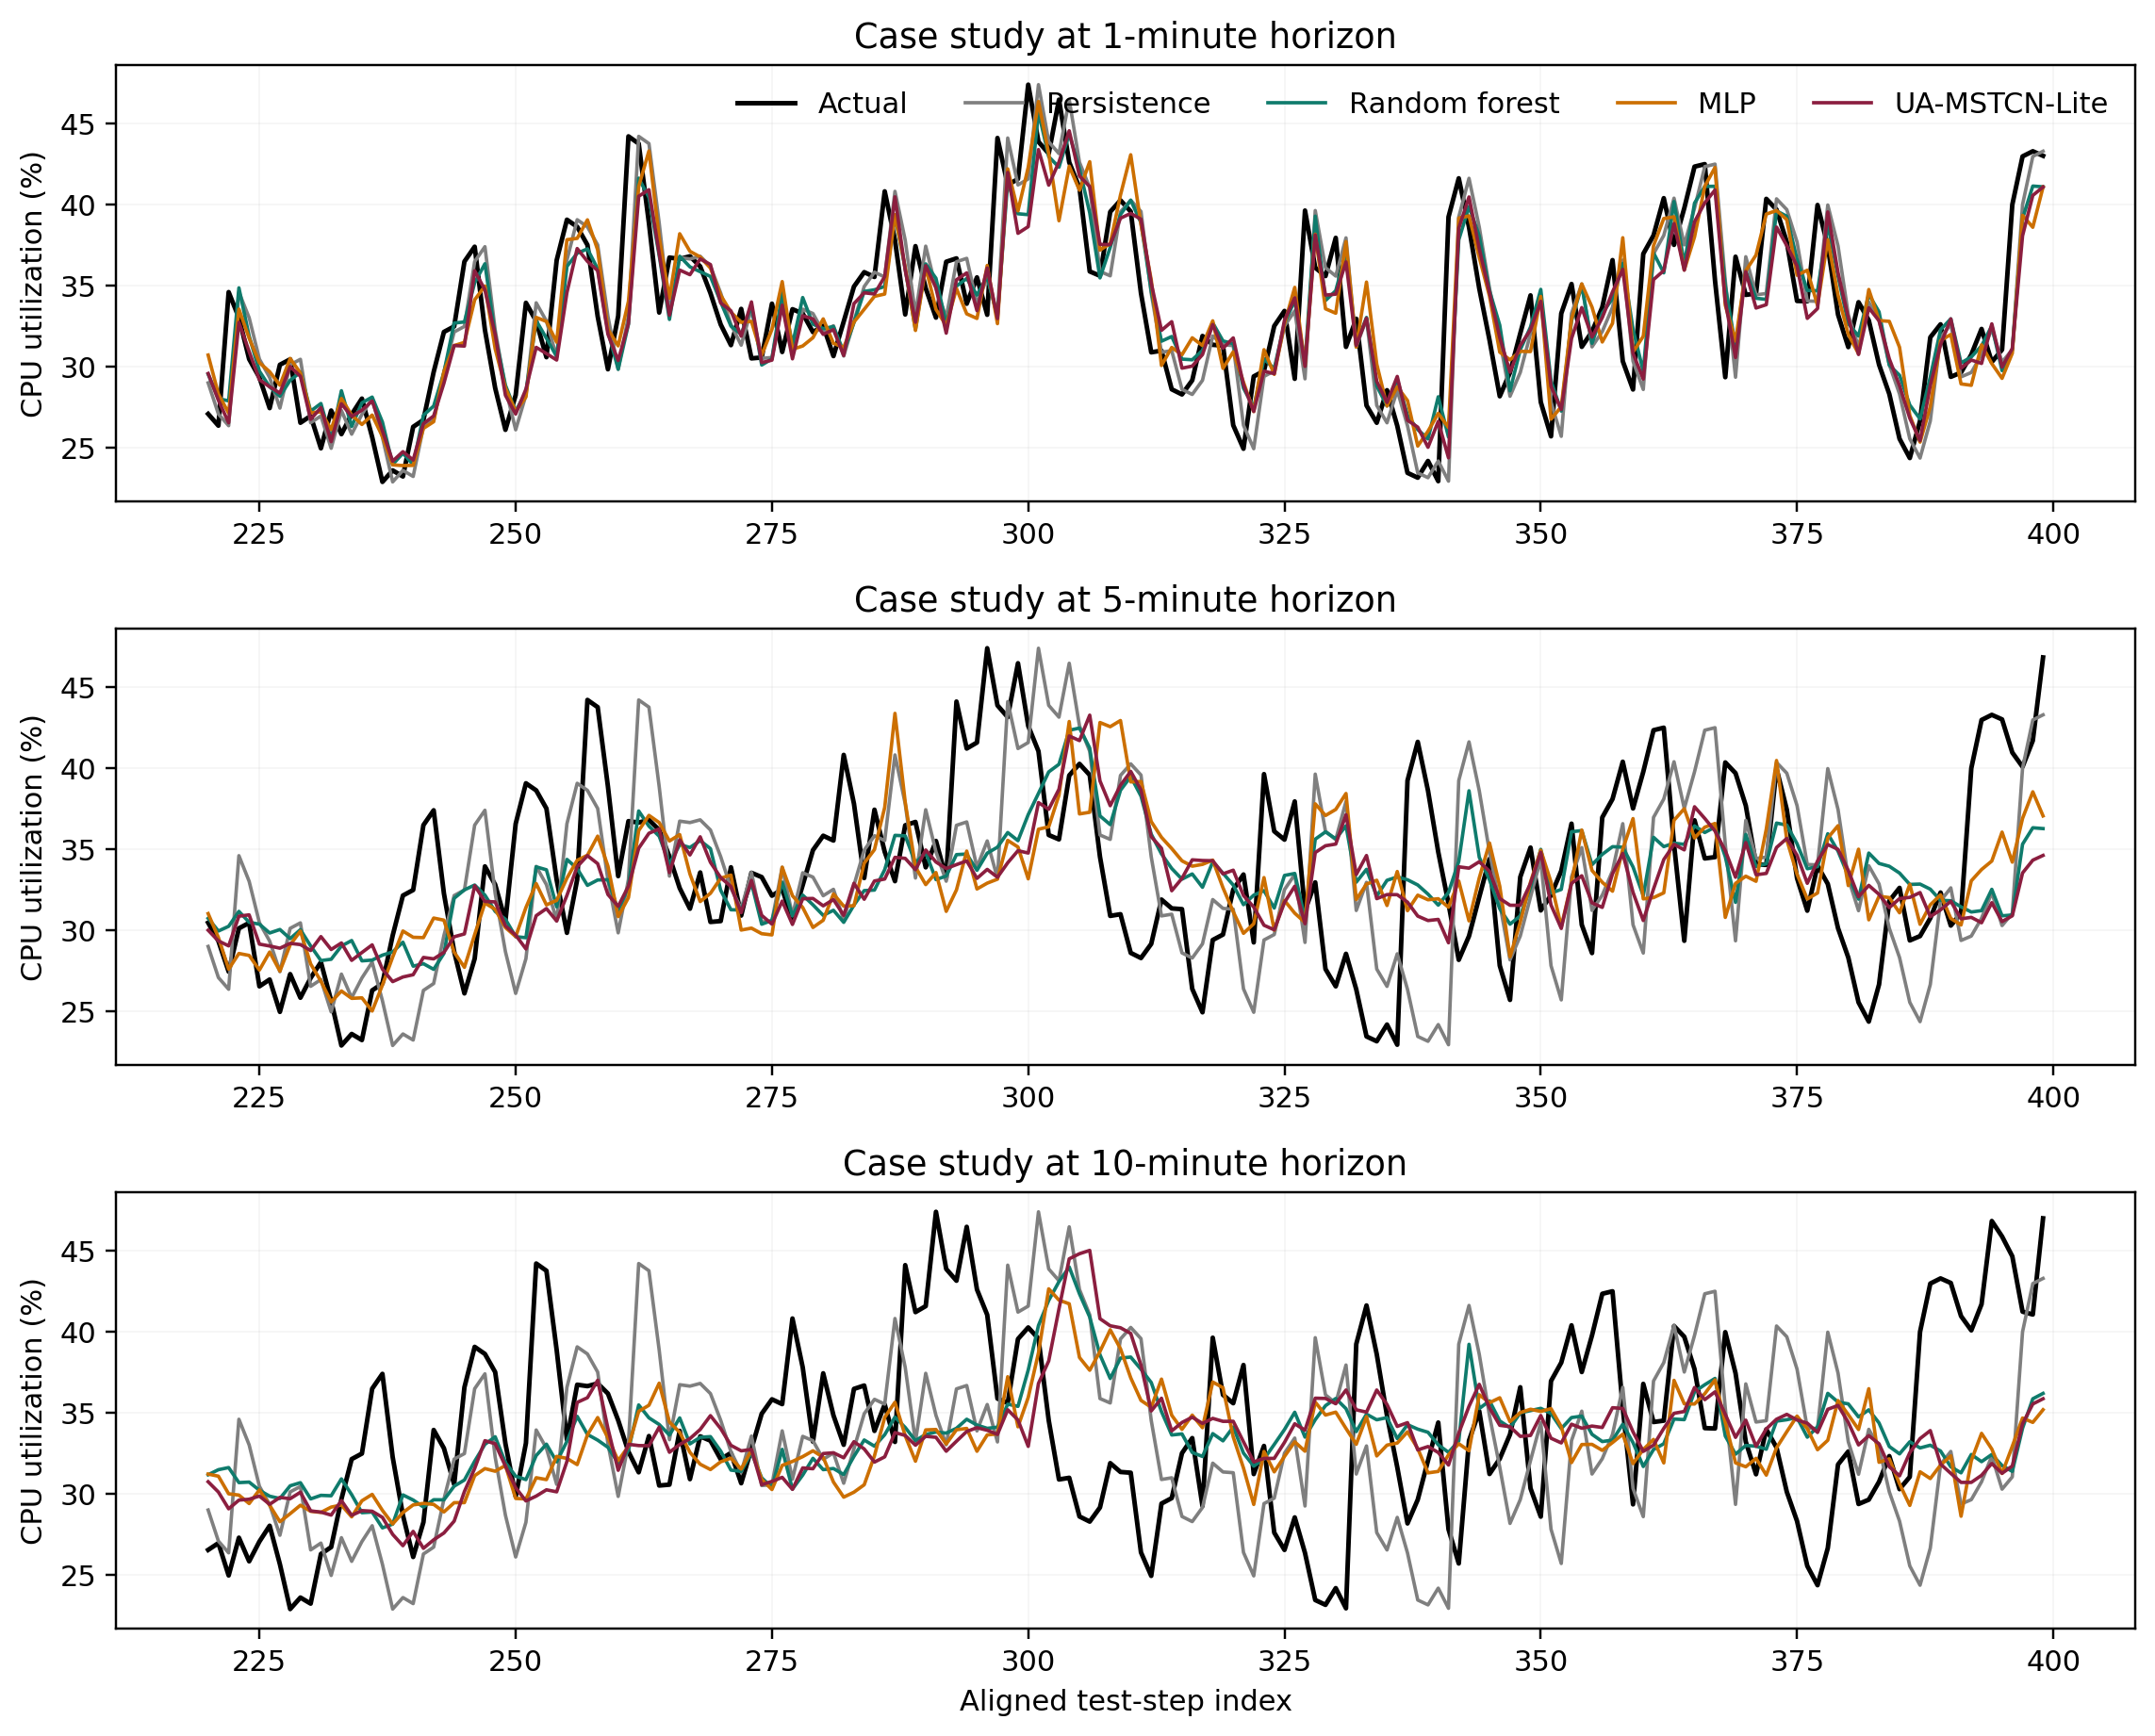
\includegraphics[width=\linewidth]{../experiments/results/figures/forecast_case_study.png}
  \caption{Forecast case study on aligned test slices for the 1-, 5-, and 10-minute horizons.}
  \label{fig:forecast-case-study}
\end{figure}

Accuracy is not the only practical concern. Figure~\ref{fig:latency-tradeoff} shows the trade-off between average MAE and average wall-clock runtime per benchmark call on the current workstation. Linear regression is now the strongest average point predictor at 19.3 ms per benchmark call, the MLP baseline sits in the middle at about 630 ms per call, random forest is slightly better in MAE than MLP but over an order of magnitude slower, and \texttt{UA-MSTCN-Lite} stays close to random forest in average MAE while also producing calibrated uncertainty estimates. This observation matters because it separates two questions that are often conflated: which model is best for point forecasting, and which model exposes the uncertainty information needed by the controller.

\begin{figure}[htbp]
  \centering
  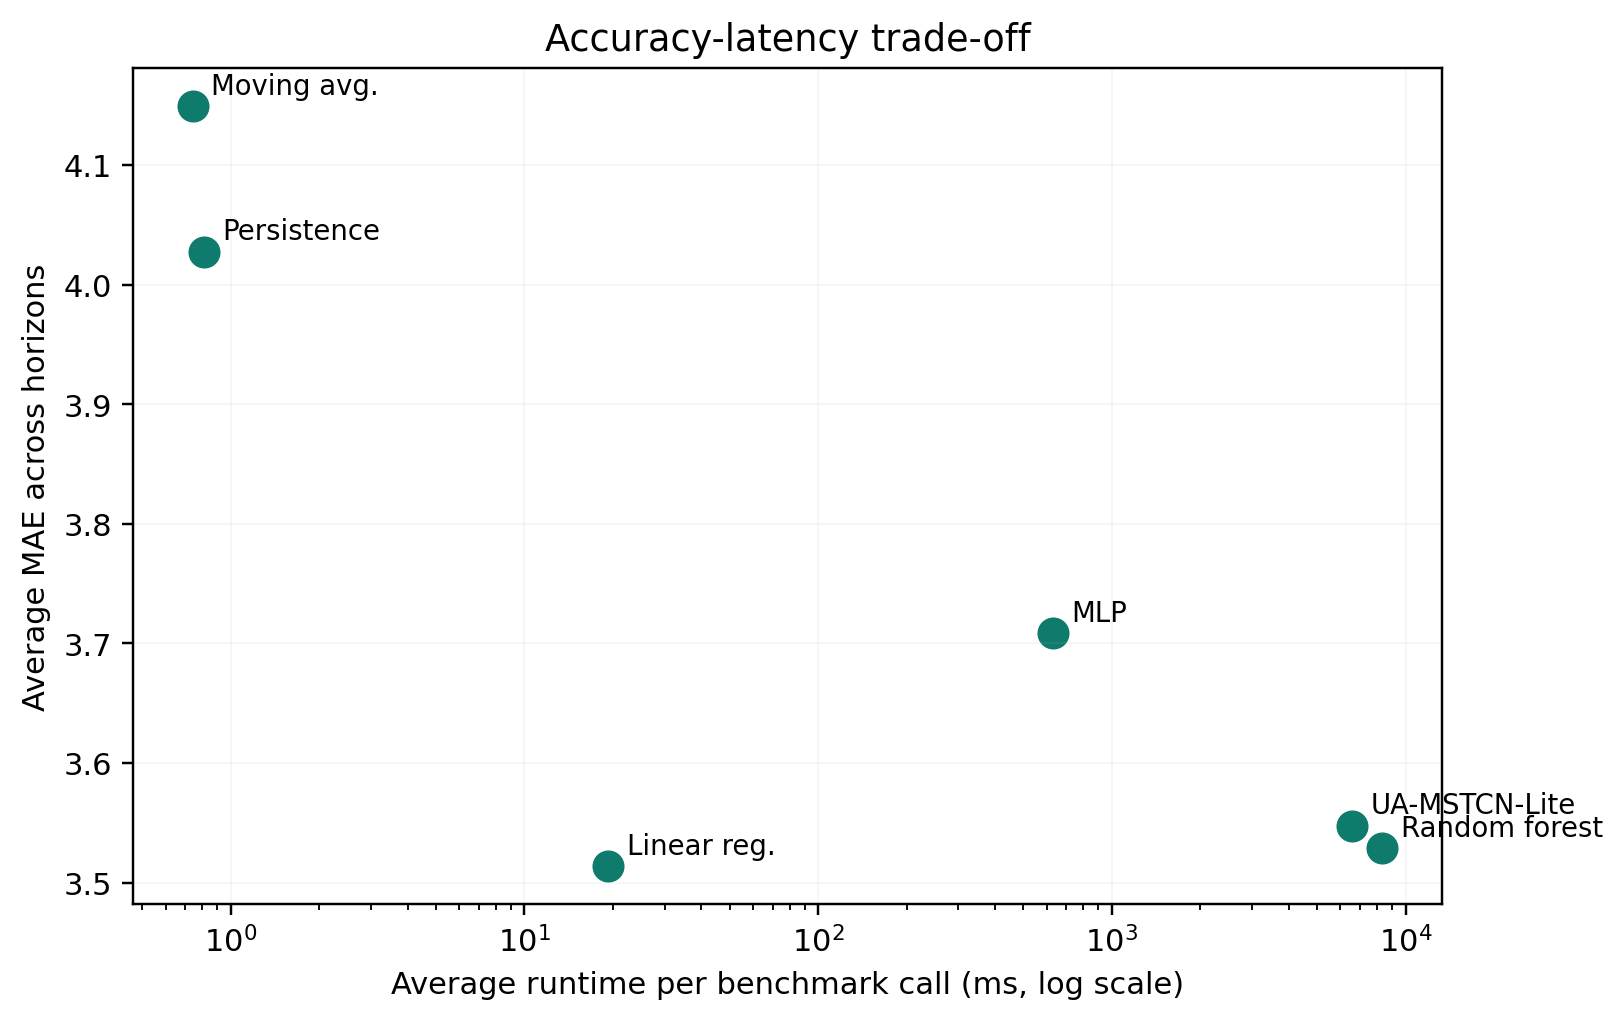
\includegraphics[width=0.82\linewidth]{../experiments/results/figures/forecast_latency_tradeoff.png}
  \caption{Average forecasting accuracy versus average runtime per benchmark call on the current workstation.}
  \label{fig:latency-tradeoff}
\end{figure}

\subsection{Context, regime, and calibration analysis}

The aggregate route also includes three forecasting diagnostics. First, Figure~\ref{fig:context-sensitivity} shows the sensitivity of \texttt{UA-MSTCN-Lite} to the context window. A 60-minute window gives the best average MAE (3.548), compared with 3.615 for 30 minutes and 3.585 for 120 minutes. The result is modest rather than dramatic, but it is still useful because it shows the default context length is not arbitrary.

\begin{figure}[htbp]
  \centering
  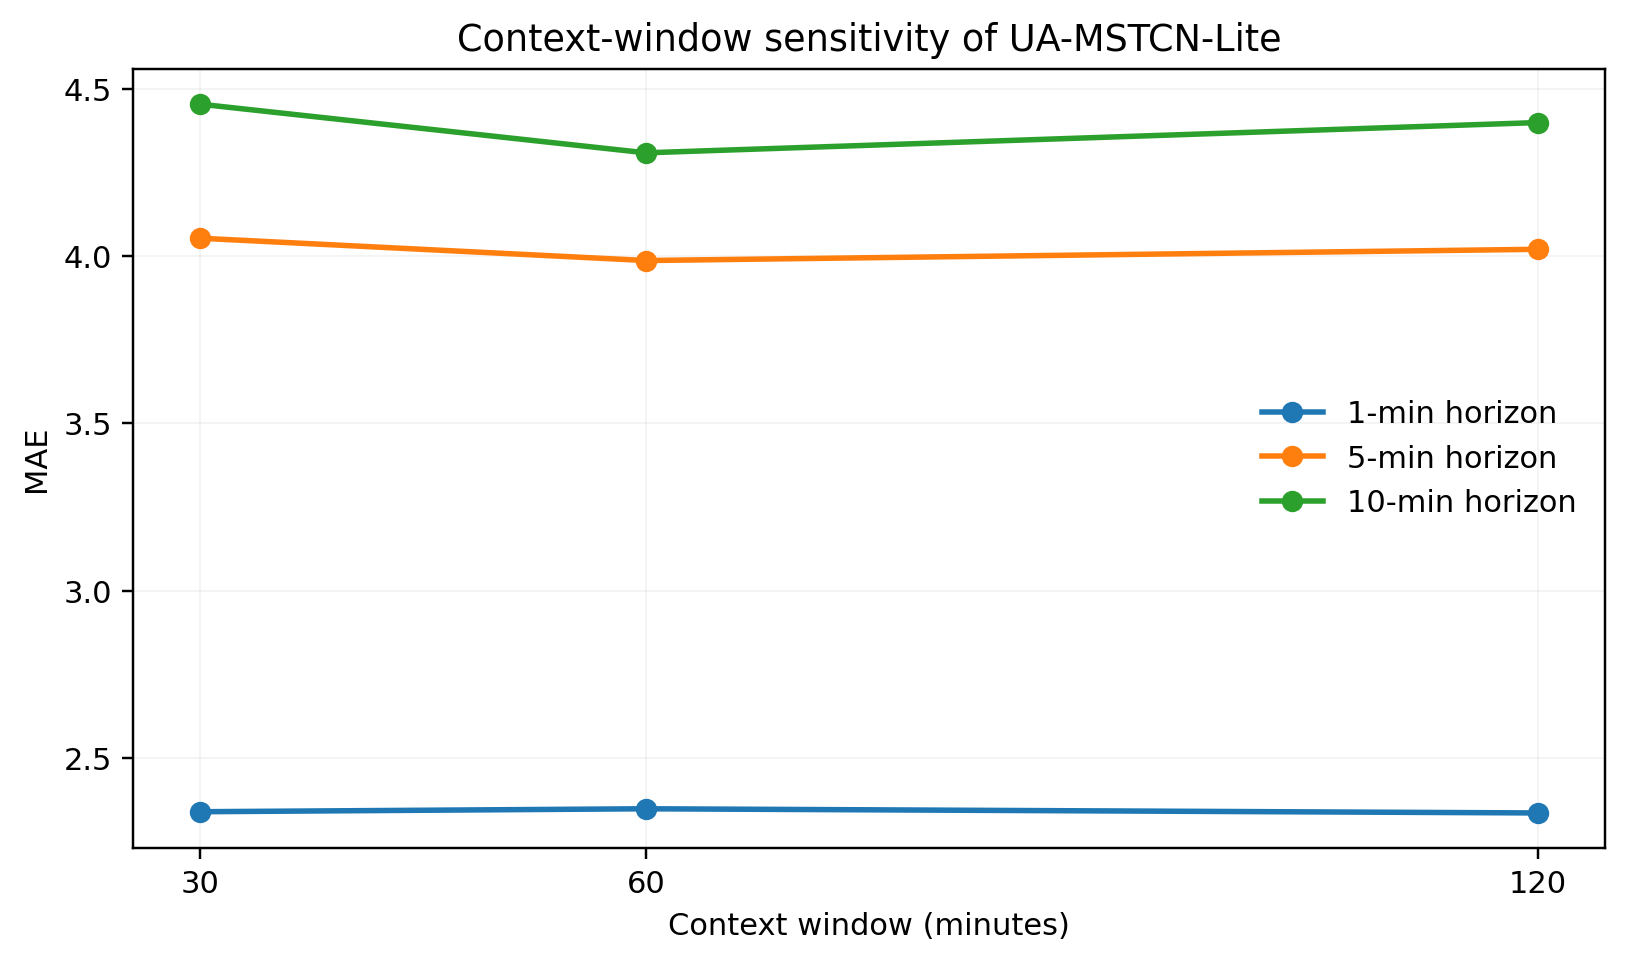
\includegraphics[width=0.76\linewidth]{../experiments/results/figures/ua_context_sensitivity.png}
  \caption{Context-window sensitivity of \texttt{UA-MSTCN-Lite}. The 60-minute default gives the best average MAE across the three evaluation horizons.}
  \label{fig:context-sensitivity}
\end{figure}

Second, Figure~\ref{fig:regime-comparison} partitions the 5-minute horizon test set into stable, moderate, and bursty regimes according to recent local volatility. The result again argues for caution rather than overclaiming: \texttt{UA-MSTCN-Lite} is slightly better than random forest in the moderate regime (3.731 vs.\ 3.752 MAE), but slightly worse in the stable and bursty regimes. This regime split shows that the surrogate is not hiding a brittle failure mode behind a single mean score, and it identifies bursty demand as the regime that most clearly needs a stronger next-generation model.

\begin{figure}[htbp]
  \centering
  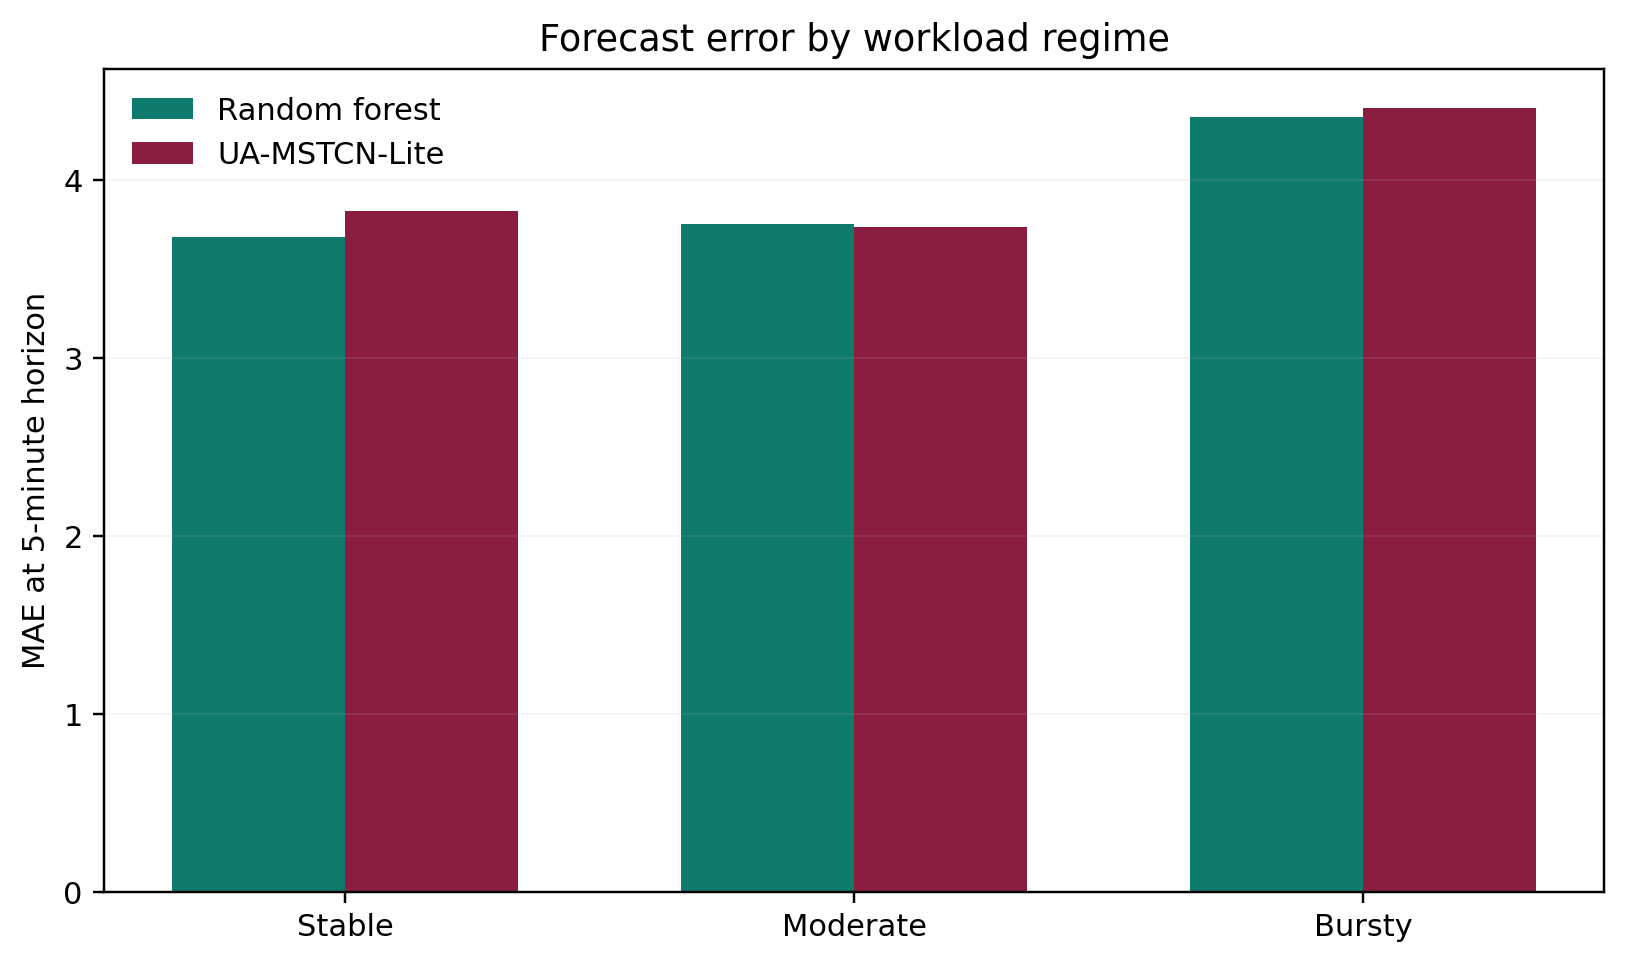
\includegraphics[width=0.76\linewidth]{../experiments/results/figures/forecast_regime_comparison.png}
  \caption{Forecast error at the 5-minute horizon across stable, moderate, and bursty workload regimes.}
  \label{fig:regime-comparison}
\end{figure}

Third, the uncertainty-aware surrogate is now evaluated directly through empirical quantile coverage. Table~\ref{tab:quantile-coverage} and Figure~\ref{fig:quantile-coverage} show that the median forecasts are well centered, with $P50$ coverage staying close to 0.5 across all horizons. The high quantile is slightly conservative at the 1-minute horizon (0.920 coverage) and mildly under-covered at the 5- and 10-minute horizons (0.867 and 0.868). This is a useful control-oriented result: the quantile band is credible enough to support a predictive policy, but the longer-horizon under-coverage explains why the controller still needs an explicit scale-out margin.

\begin{table}[htbp]
  \centering
  \caption{Empirical quantile coverage of \texttt{UA-MSTCN-Lite} on the aggregate test split.}
  \label{tab:quantile-coverage}
  \scriptsize
  \setlength{\tabcolsep}{3pt}
  \renewcommand{\arraystretch}{0.96}
  \begin{tabular}{lccc}
    \toprule
    Horizon & $P50$ cov. & $P90$ cov. & Mean int. width \\
    \midrule
    1 minute & 0.506 & 0.920 & 4.623 \\
    5 minutes & 0.516 & 0.867 & 6.709 \\
    10 minutes & 0.500 & 0.868 & 7.405 \\
    \bottomrule
  \end{tabular}
\end{table}

\begin{figure}[htbp]
  \centering
  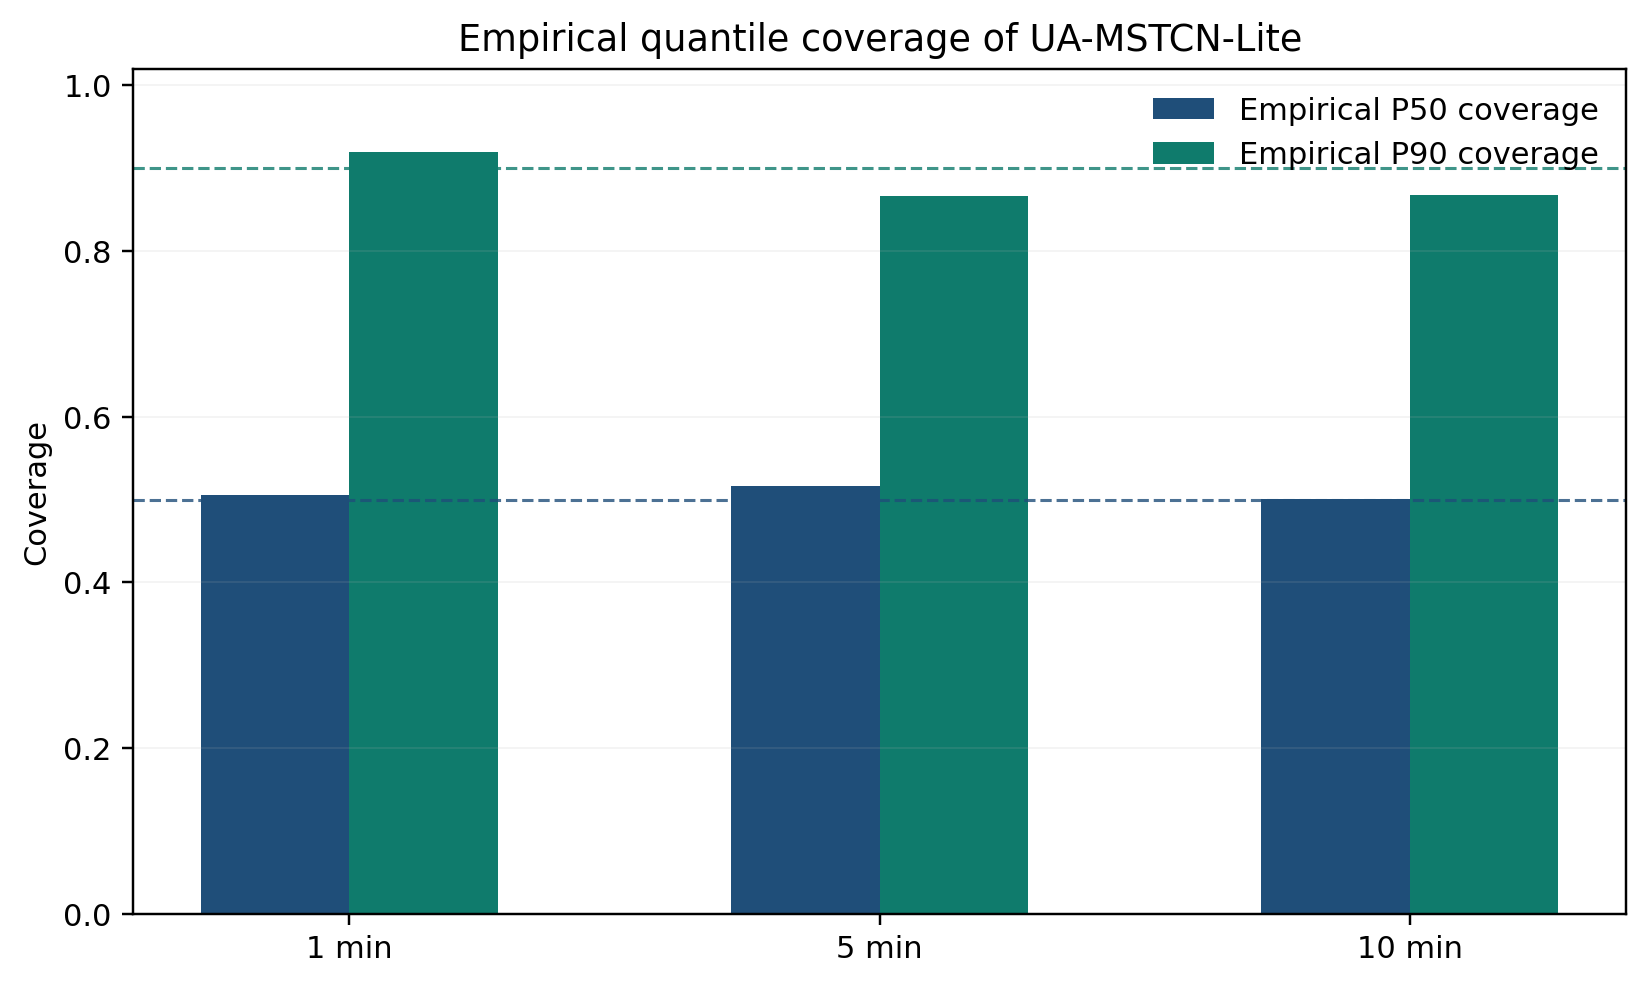
\includegraphics[width=0.72\linewidth]{../experiments/results/figures/quantile_coverage.png}
  \caption{Empirical $P50$ and $P90$ coverage of \texttt{UA-MSTCN-Lite}. Dashed lines indicate the nominal target levels.}
  \label{fig:quantile-coverage}
\end{figure}

\subsection{Cross-entity machine-cohort benchmark}

The aggregate trace is no longer the only evidence surface. A second benchmark extracted from 12 high-coverage machines tests whether the forecasting story changes once the unit of analysis shifts from one cluster-wide series to multiple long-lived entities. Table~\ref{tab:machine-cohort-summary} summarizes the average error across the cohort. The qualitative ranking is stable and, if anything, harsher on the surrogate than the aggregate benchmark: linear regression is the strongest point predictor at every horizon, with mean MAE values of 3.633, 5.520, and 5.966. The standard neural MLP baseline becomes the second-best average point predictor at all three horizons (3.921, 5.845, and 6.301), but it still trails linear regression by 0.29--0.34 MAE. \texttt{UA-MSTCN-Lite} remains close to random forest and now trails even the simple MLP baseline on this cohort.

\begin{table}[htbp]
  \centering
  \caption{Average forecasting performance across the 12-machine high-coverage cohort.}
  \label{tab:machine-cohort-summary}
  \tiny
  \setlength{\tabcolsep}{2pt}
  \renewcommand{\arraystretch}{0.95}
  \begin{tabular}{lcccc}
    \toprule
    Model & H & MAE & RMSE & MAPE \\
    \midrule
    Persistence & 1 & 3.716 & 5.185 & 0.103 \\
    Linear regression & 1 & 3.633 & 4.926 & 0.101 \\
    MLP regressor & 1 & 3.921 & 5.246 & 0.109 \\
    Random forest & 1 & 4.012 & 5.396 & 0.107 \\
    UA-MSTCN-Lite & 1 & 4.121 & 5.647 & 0.106 \\
    Persistence & 5 & 6.268 & 8.497 & 0.172 \\
    Linear regression & 5 & 5.520 & 7.318 & 0.153 \\
    MLP regressor & 5 & 5.845 & 7.683 & 0.159 \\
    Random forest & 5 & 6.170 & 8.223 & 0.162 \\
    UA-MSTCN-Lite & 5 & 6.244 & 8.423 & 0.161 \\
    Persistence & 10 & 6.932 & 9.390 & 0.192 \\
    Linear regression & 10 & 5.966 & 7.959 & 0.165 \\
    MLP regressor & 10 & 6.301 & 8.324 & 0.172 \\
    Random forest & 10 & 6.548 & 8.745 & 0.173 \\
    UA-MSTCN-Lite & 10 & 6.651 & 8.936 & 0.172 \\
    \bottomrule
  \end{tabular}
\end{table}

Figure~\ref{fig:machine-cohort-mae} makes the same pattern easier to scan. Linear regression wins 6, 8, and 8 of the 12 entities at the 1-, 5-, and 10-minute horizons, respectively. The MLP baseline wins no machine-horizon cell, which shows that its gain over random forest and \texttt{UA-MSTCN-Lite} comes from broad but modest improvements rather than from dominant wins on specific entities. \texttt{UA-MSTCN-Lite} still wins only 2, 3, and 2 entities across these horizons. This is exactly the kind of result that should remain in the manuscript instead of being optimized away: it shows that the current surrogate is not yet the strongest general-purpose point forecaster when the workload granularity becomes finer.

\begin{figure}[htbp]
  \centering
  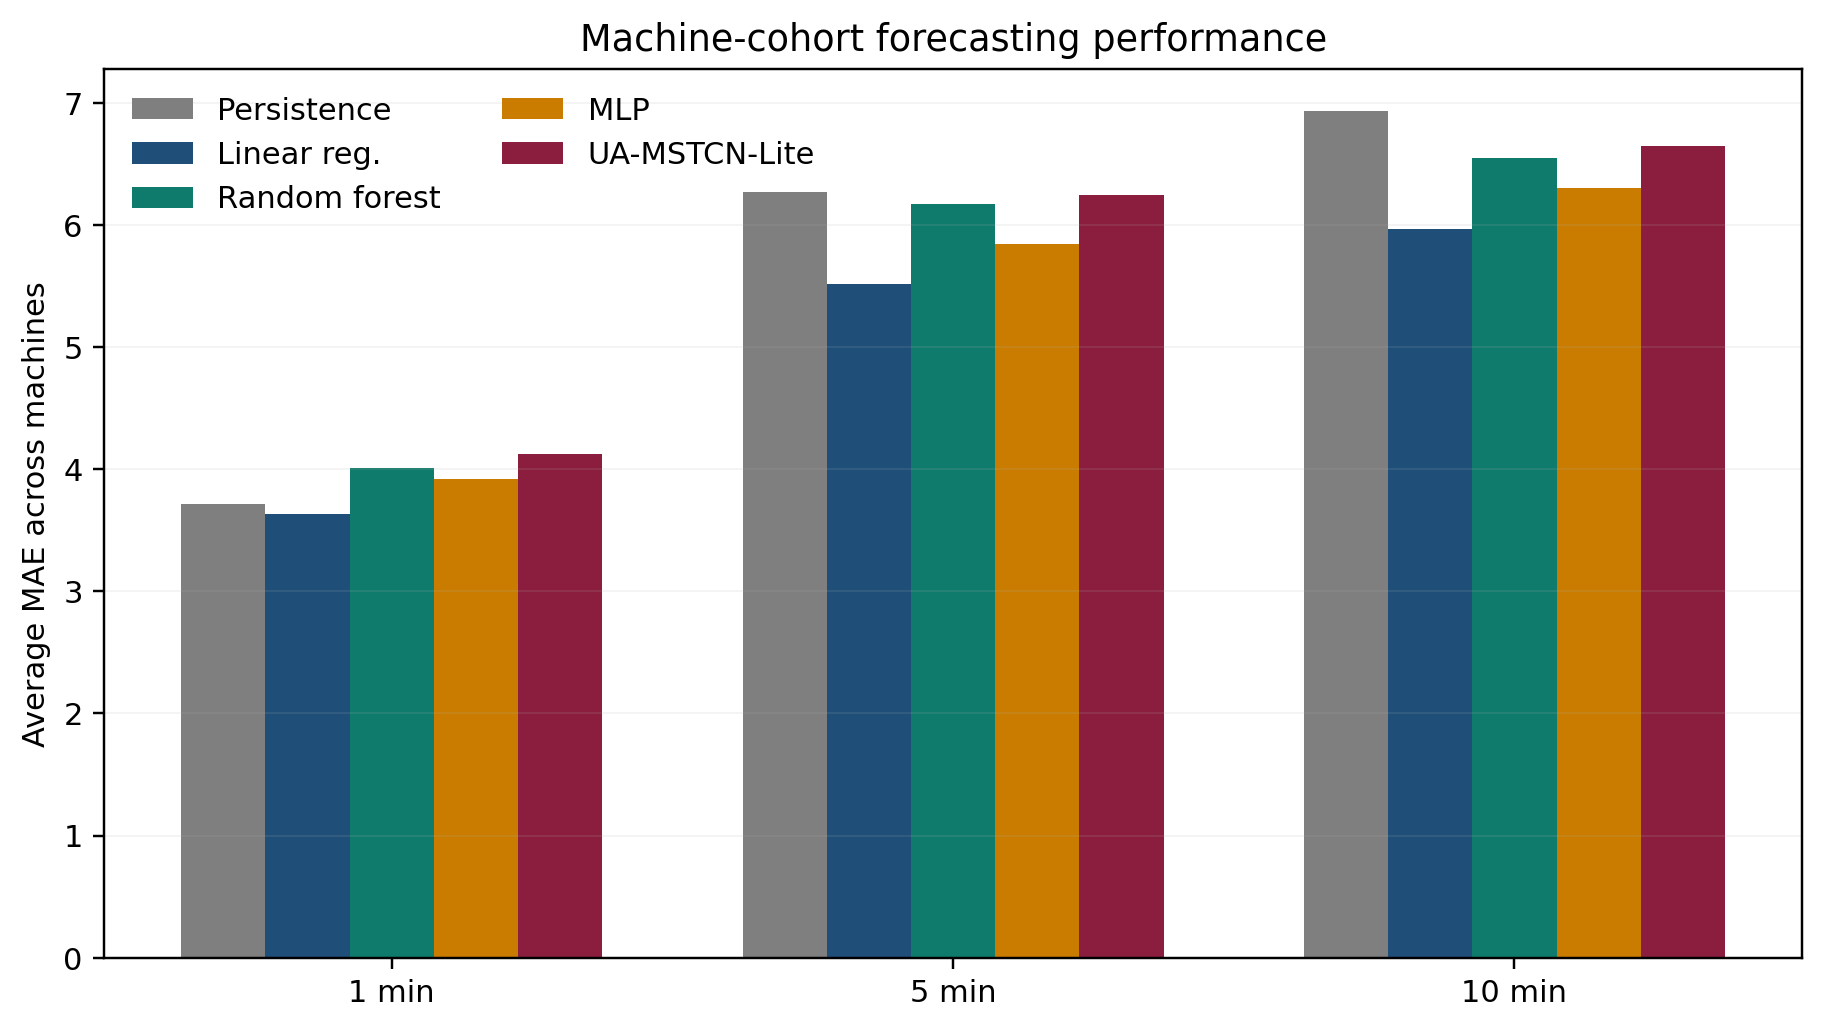
\includegraphics[width=0.78\linewidth]{../experiments/results/machine_cohort/figures/machine_cohort_mae_by_horizon.png}
  \caption{Average forecasting MAE across the 12-machine high-coverage cohort.}
  \label{fig:machine-cohort-mae}
\end{figure}

Figure~\ref{fig:machine-cohort-entity} adds one more view of this heterogeneity. For most machines, \texttt{UA-MSTCN-Lite} remains fairly close to linear regression, but a small subset of entities drives most of the gap. The worst case in the current cohort is \texttt{m\_2014}, where the surrogate's average MAE reaches 9.37 compared with 6.04 for linear regression. This heterogeneity identifies where a deeper temporal model would earn its keep.

\begin{figure}[htbp]
  \centering
  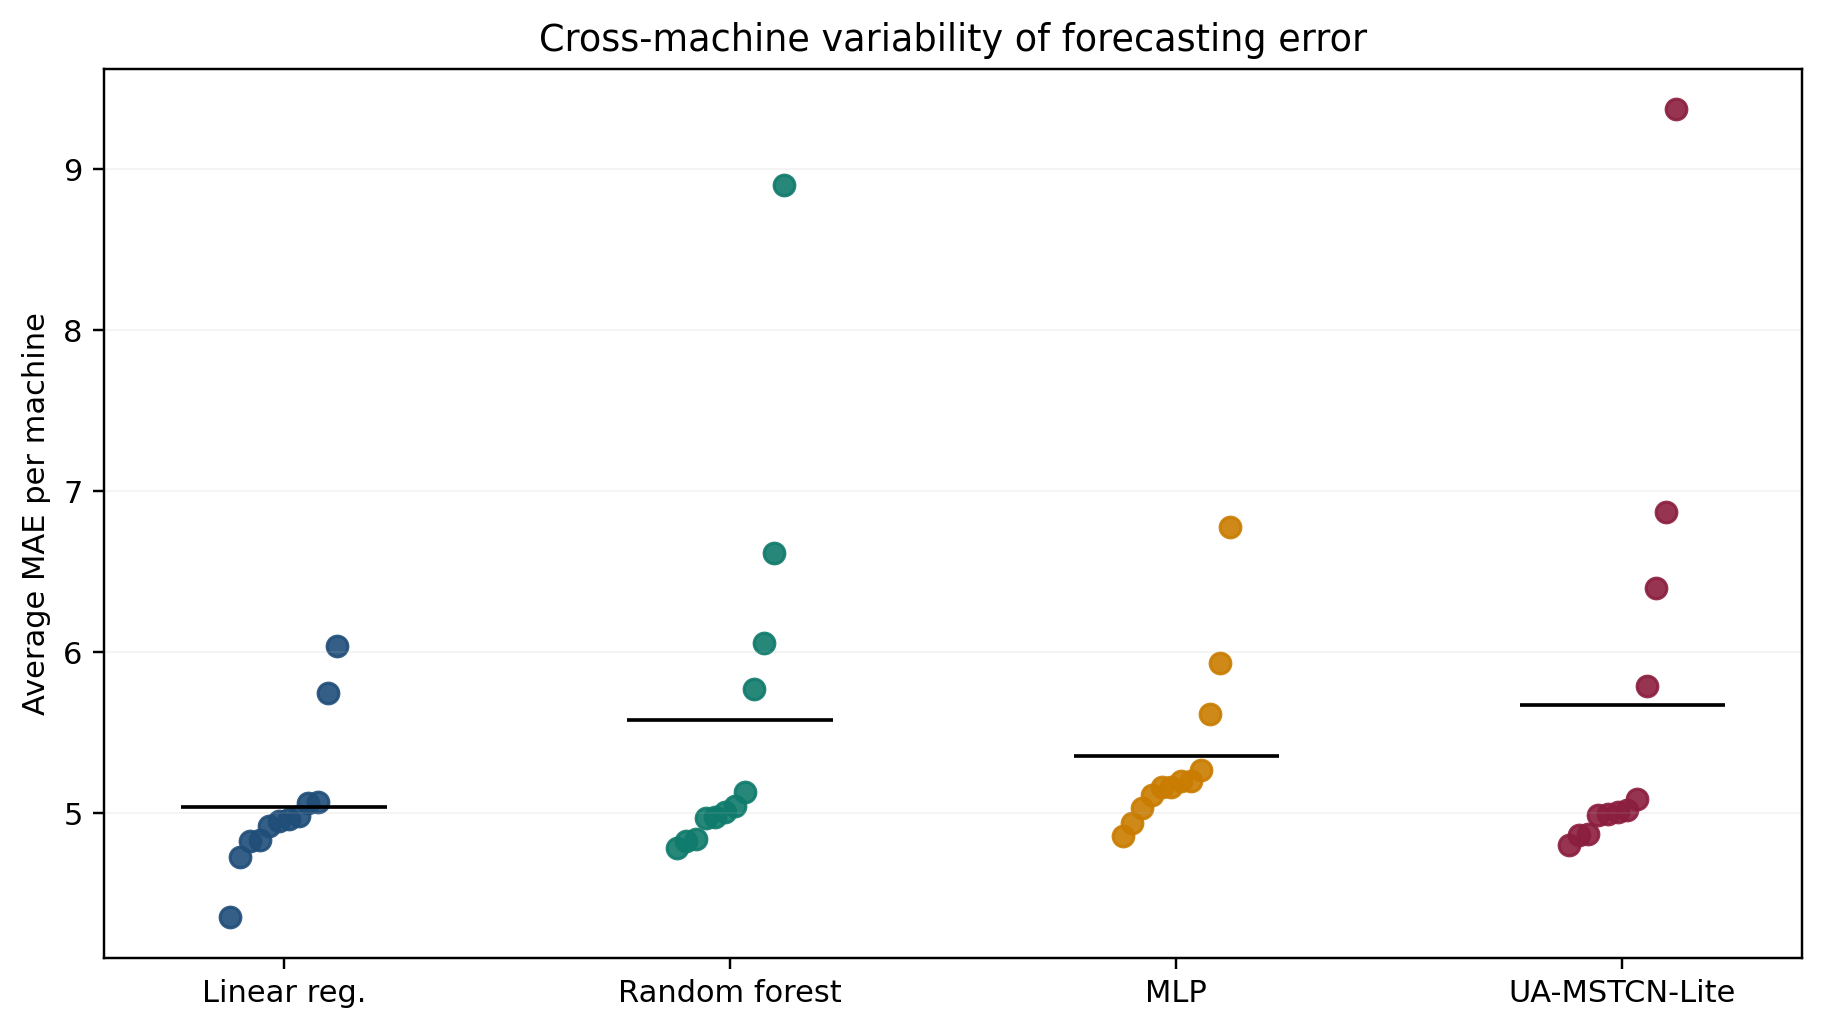
\includegraphics[width=0.78\linewidth]{../experiments/results/machine_cohort/figures/machine_cohort_entity_mae.png}
  \caption{Per-machine average MAE across the 12-machine cohort. Each point is one machine and the horizontal segment marks the model mean.}
  \label{fig:machine-cohort-entity}
\end{figure}

The machine-cohort experiment still supports the uncertainty-aware part of the paper. Table~\ref{tab:machine-cohort-coverage} shows that average $P50$ coverage stays close to 0.5 across horizons and average $P90$ coverage stays between 0.847 and 0.891. The longer-horizon under-coverage is therefore not unique to the aggregate benchmark. This cross-entity pattern strengthens the interpretation that the predictive controller genuinely benefits from an explicit scale-out margin rather than receiving one only as a patch for a single series.

\begin{table}[htbp]
  \centering
  \caption{Average quantile coverage of \texttt{UA-MSTCN-Lite} across the 12-machine cohort.}
  \label{tab:machine-cohort-coverage}
  \scriptsize
  \setlength{\tabcolsep}{3pt}
  \renewcommand{\arraystretch}{0.96}
  \begin{tabular}{lccc}
    \toprule
    Horizon & $P50$ cov. & $P90$ cov. & Mean int. width \\
    \midrule
    1 minute & 0.510 & 0.891 & 7.529 \\
    5 minutes & 0.523 & 0.853 & 9.375 \\
    10 minutes & 0.517 & 0.847 & 9.825 \\
    \bottomrule
  \end{tabular}
\end{table}

\begin{figure}[htbp]
  \centering
  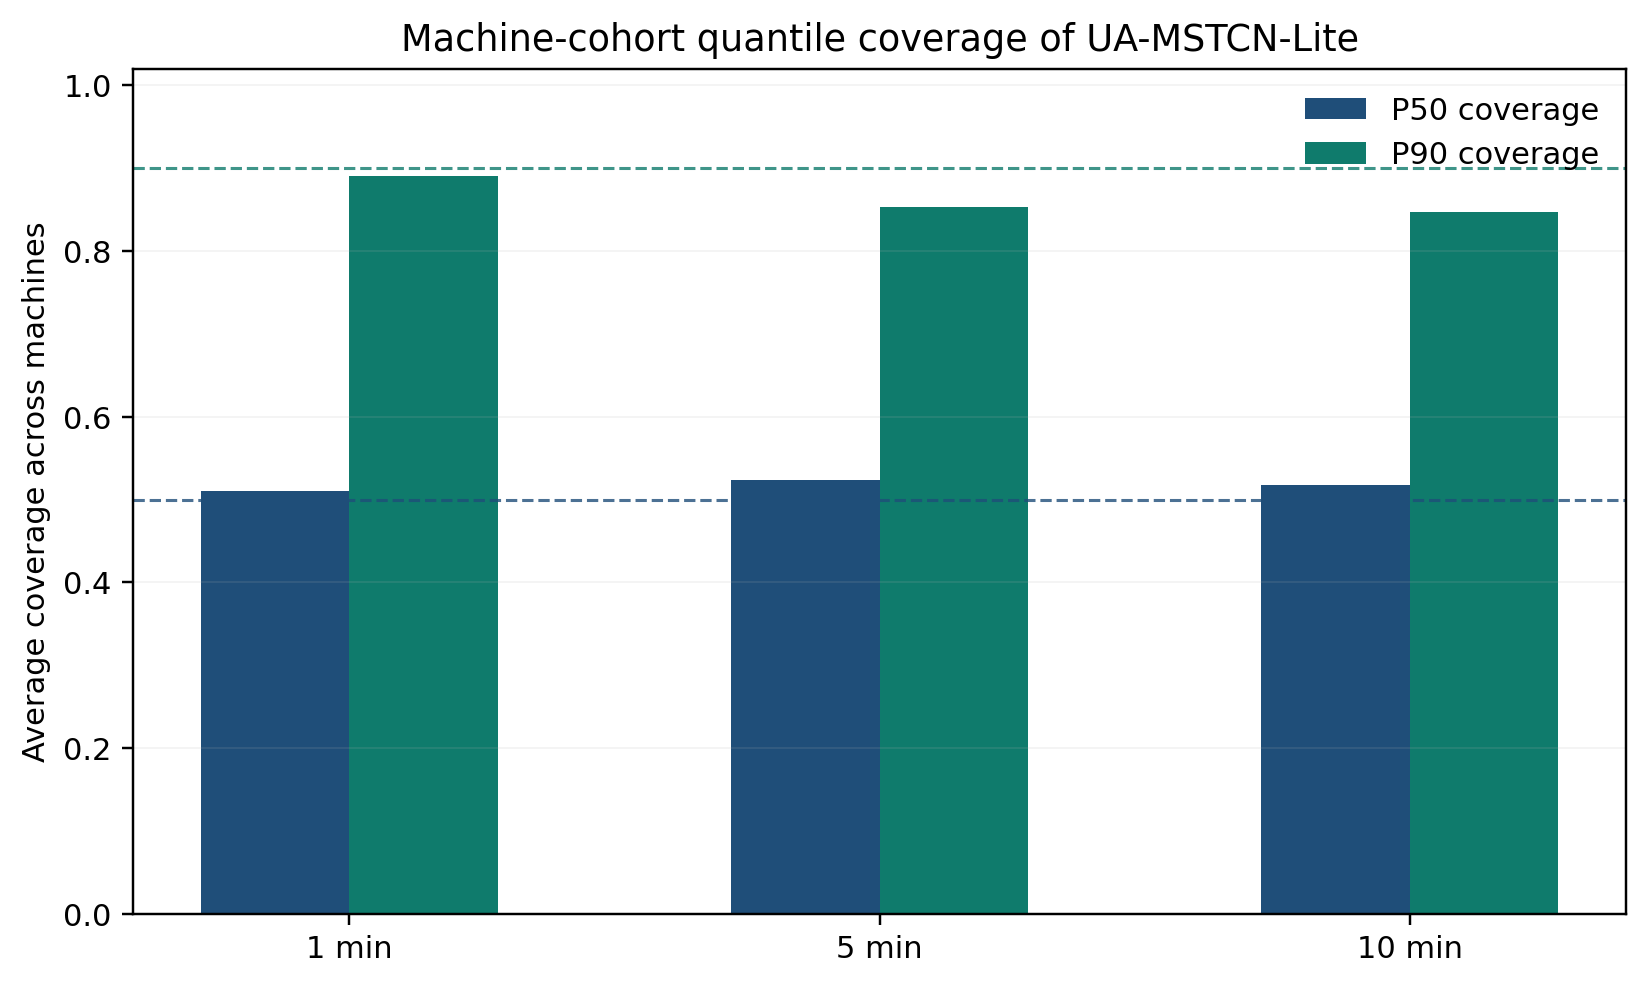
\includegraphics[width=0.72\linewidth]{../experiments/results/machine_cohort/figures/machine_cohort_quantile_coverage.png}
  \caption{Average $P50$ and $P90$ coverage of \texttt{UA-MSTCN-Lite} across the 12-machine cohort.}
  \label{fig:machine-cohort-coverage}
\end{figure}

\subsection{Cross-machine transfer}

The next question is whether forecasting structure learned from one set of machines transfers to unseen machines. To test this, the study runs a 3-fold zero-shot transfer benchmark on the same 12-machine cohort. In each fold, 8 machines are used to train pooled global models and 4 machines are held out entirely for evaluation. Table~\ref{tab:machine-transfer} summarizes the result.

\begin{table}[htbp]
  \centering
  \caption{Cross-machine zero-shot transfer on held-out machines.}
  \label{tab:machine-transfer}
  \tiny
  \setlength{\tabcolsep}{1pt}
  \renewcommand{\arraystretch}{0.96}
  \begin{tabular}{lcccccc}
    \toprule
    Horizon & Pers. & Glob. lin. & Glob. MLP & Glob. RF & Glob. UA & Ent. lin. \\
    \midrule
    1 minute & 3.716 & 3.629 & 3.735 & 4.496 & 3.934 & 3.633 \\
    5 minutes & 6.268 & 5.503 & 5.722 & 6.293 & 6.328 & 5.520 \\
    10 minutes & 6.932 & 5.953 & 6.286 & 6.642 & 6.648 & 5.966 \\
    \bottomrule
  \end{tabular}
\end{table}

The most important observation is not about the uncertainty-aware surrogate. It is that pooled linear regression transfers extremely well across machines. Its mean MAE differs from the entity-specific linear upper bound by only $-0.004$, $-0.017$, and $-0.013$ at the 1-, 5-, and 10-minute horizons, respectively. In other words, the held-out machines in this cohort share enough temporal structure that a simple global linear model generalizes almost perfectly. The global MLP baseline is the next-best zero-shot point predictor, with mean MAE 3.735, 5.722, and 6.286, but it still trails global linear regression at every horizon. This result sets a strong and transparent transfer baseline instead of assuming that a more complex model should dominate by default.

The global \texttt{UA-MSTCN-Lite} model does not beat that baseline on point accuracy, but it still contributes transferable uncertainty estimates. Across held-out machines, its average $P90$ coverage is 0.904, 0.859, and 0.853 for the 1-, 5-, and 10-minute horizons. The same pattern seen in the aggregate and per-machine benchmarks therefore remains visible under zero-shot transfer: point-prediction leadership belongs to the linear baseline, while the uncertainty-aware surrogate remains useful because it exports calibrated quantile bands that a controller can consume.

\begin{figure}[htbp]
  \centering
  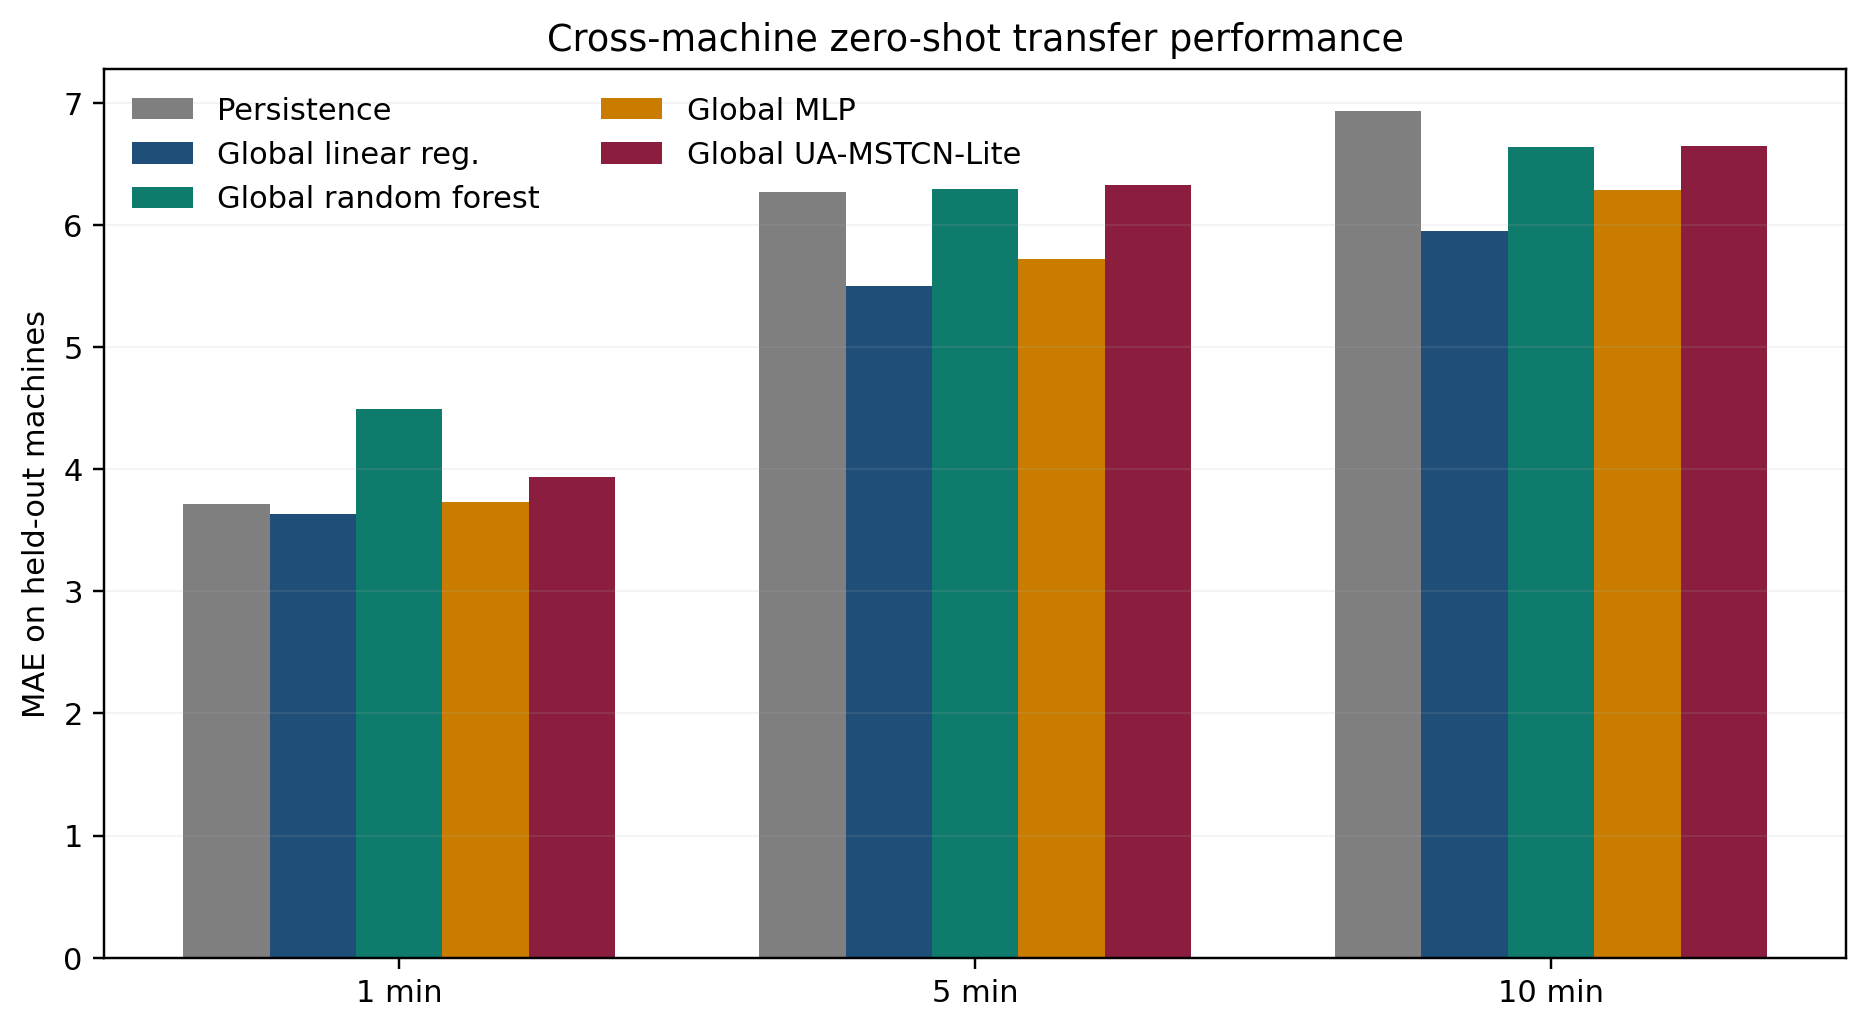
\includegraphics[width=0.78\linewidth]{../experiments/results/machine_transfer/figures/machine_transfer_zero_shot_mae.png}
  \caption{Cross-machine zero-shot transfer performance across the 3 deterministic folds.}
  \label{fig:machine-transfer}
\end{figure}

\subsection{Container service-level evidence}

The construct-validity gap is now materially narrower because the evaluation no longer stops at aggregate and machine abstractions. Using the official \texttt{container\_meta} table together with a full mirrored pass over \texttt{container\_usage}, the study builds a broad service-level cohort covering 139 \texttt{app\_du} groups, 19{,}419 selected containers, 19{,}269 matched containers, and the full shared 11{,}520-minute span introduced in Section~4. A dedicated overlap audit retains all 10 services from the earlier targeted cohort, and the broader audited selection materially changes the service-level conclusions. Table~\ref{tab:service-cohort-promotion} shows that broader service coverage shifts the forecasting winner from \texttt{UA-MSTCN-Lite} to linear regression, turns the scaling-actions delta positive, and leaves the apparent over-provisioning gain unsupported under paired service bootstrap.

\begin{table}[htbp]
  \centering
  \caption{Comparison of service-level conclusions under the earlier targeted top-10 cohort and the broader audited cohort. Deltas are equal-weighted predictive-minus-reactive means.}
  \label{tab:service-cohort-promotion}
  \scriptsize
  \setlength{\tabcolsep}{2pt}
  \renewcommand{\arraystretch}{0.96}
  \begin{tabular}{lcccccc}
    \toprule
    Cohort & Svcs & Cov. & Winner & SLA $\Delta$ & Over $\Delta$ & Acts $\Delta$ \\
    \midrule
    Top-10 & 10 & 0.971 & UA-Lite & +0.033 & -0.720 & -52.4 \\
    Broad & 139 & 0.973 & Linear & +0.014 & -2.633 & +150.4 \\
    \bottomrule
  \end{tabular}
\end{table}

Table~\ref{tab:service-forecasting-summary} summarizes the forecasting result on the audited broad cohort. Linear regression is strongest at every horizon, with MAE 19.999, 34.250, and 43.463 at the 1-, 5-, and 10-minute horizons, respectively. Persistence becomes the overall runner-up at 33.381 average MAE, which is itself a useful warning that local continuity remains a very strong service-level baseline under the broader selection rule. The standard neural MLP baseline does not change that ranking: its average MAE is 37.066, ahead of \texttt{UA-MSTCN-Lite} at 37.787 but behind both linear regression and persistence. The narrower targeted cohort had favored \texttt{UA-MSTCN-Lite}, but that ranking does not survive broader audited service coverage.

\begin{table}[htbp]
  \centering
  \caption{Service-level forecasting across the audited 139-service \texttt{app\_du} cohort.}
  \label{tab:service-forecasting-summary}
  \scriptsize
  \setlength{\tabcolsep}{2pt}
  \renewcommand{\arraystretch}{0.96}
  \begin{tabular}{lcccc}
    \toprule
    Model & 1 min. & 5 min. & 10 min. & Avg. \\
    \midrule
    Persistence & 20.408 & 34.638 & 45.098 & 33.381 \\
    Linear regression & 19.999 & 34.250 & 43.463 & 32.571 \\
    MLP regressor & 23.684 & 38.395 & 49.117 & 37.066 \\
    Random forest & 26.317 & 37.728 & 44.912 & 36.319 \\
    UA-MSTCN-Lite & 27.939 & 39.746 & 45.677 & 37.787 \\
    \bottomrule
  \end{tabular}
\end{table}

Figure~\ref{fig:service-forecasting} shows the same result visually. The more interesting interpretation is not simply that a different model wins. It is that the service traces are much less homogeneous than the aggregate or machine cohorts, and once the selection widens enough, that heterogeneity no longer favors the uncertainty-aware surrogate on point accuracy. This is precisely why a broader service-level extension matters: it reveals that service-level conclusions based on a small targeted subset can move materially once the selection rule is widened and audited.

\begin{figure}[htbp]
  \centering
  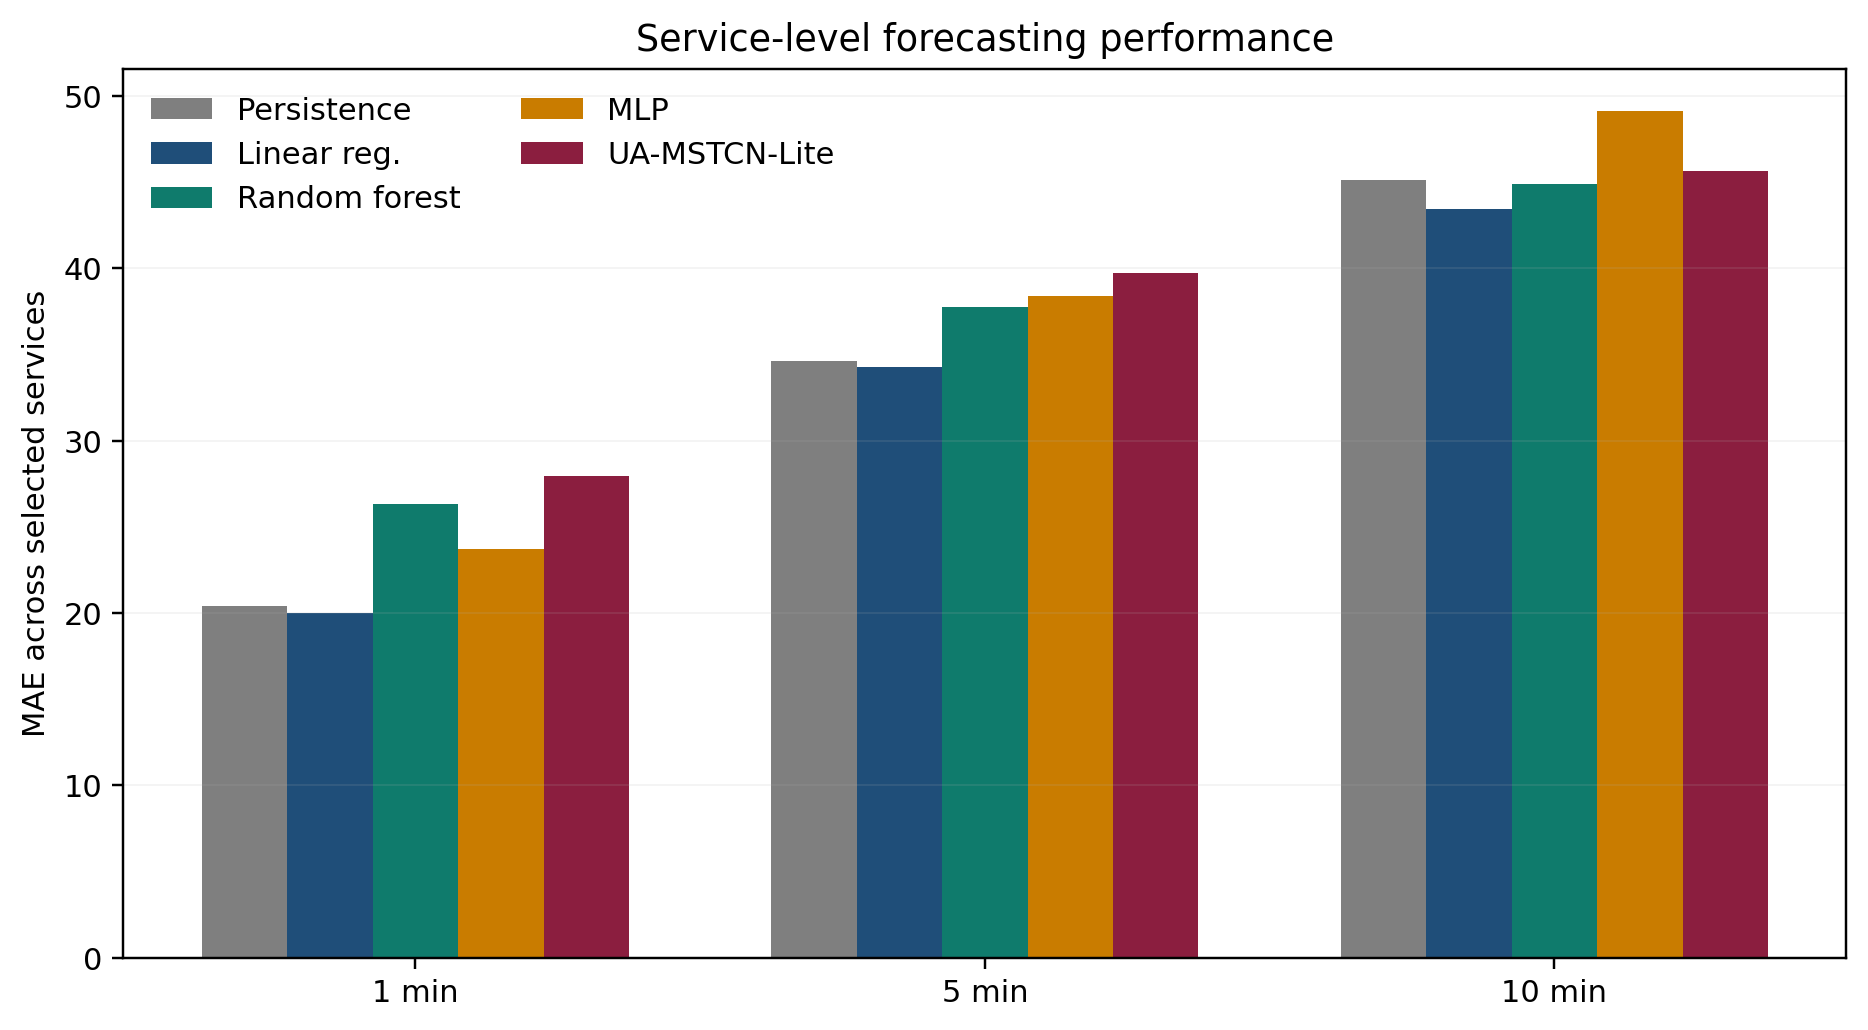
\includegraphics[width=0.82\linewidth]{../experiments/results/service_cohort_broad/figures/service_forecasting_mae.png}
  \caption{Average MAE across the audited 139-service \texttt{app\_du} cohort. Under broader service coverage, point-forecast leadership shifts to linear regression and the generic MLP baseline remains mid-pack rather than dominant.}
  \label{fig:service-forecasting}
\end{figure}

The quantile behavior also remains useful at this finer granularity. Across the 139 services, the empirical $P90$ coverage of \texttt{UA-MSTCN-Lite} is 0.921, 0.896, and 0.877 at the 1-, 5-, and 10-minute horizons, respectively. The median forecasts remain slightly under-centered, with $P50$ coverage between 0.469 and 0.481, but the upper quantile stays close enough to the nominal target to justify its continued use inside the predictive controller even though the model no longer leads on point MAE.

The service-level control comparison is more stringent than the aggregate result because it evaluates the policy under heterogeneous service demand rather than one shared cluster signal. Averaged over the 139 services, the forecast-free lagged target-tracking baseline again marks one extreme of the trade-off surface: it drives over-provisioning down to 3.848 and average reserved capacity down to 124.046, but SLA violation rises to 0.486 and scaling actions explode to 1660.9. Against the operational reactive baseline, the predictive controller raises mean SLA violation from 0.0173 to 0.0311, raises mean scaling actions from 249.0 to 399.4, and raises mean reserved capacity from 164.484 to 178.008, while mean over-provisioning falls from 56.310 to 53.677. The paired service bootstrap makes the conclusion sharper. The equal-weighted predictive-minus-reactive SLA delta is +0.0138 with a 95\% interval of [0.0035, 0.0271], which is a stable degradation. The equal-weighted scaling-actions delta is +150.4 with interval [114.0, 185.0], another stable degradation. The equal-weighted over-provisioning delta remains negative at -2.633, but its interval [-6.953, 2.328] crosses zero, so the apparent over-provisioning gain is not stably supportable under broader service resampling. The auxiliary load-weighted mean scaling-actions delta is nearly zero (-0.567) and also not stable, which suggests that the equal-weighted penalty is driven more by widespread small-service regressions than by the highest-load services alone. At the per-service level, predictive control improves SLA violation for only 27 of 139 services and reduces scaling actions for only 32 of 139, even though it reduces over-provisioning for 95 services. These mixed and negative findings are not incidental; they identify the boundary conditions under which a shared global predictive policy fails under service heterogeneity.

\begin{figure}[htbp]
  \centering
  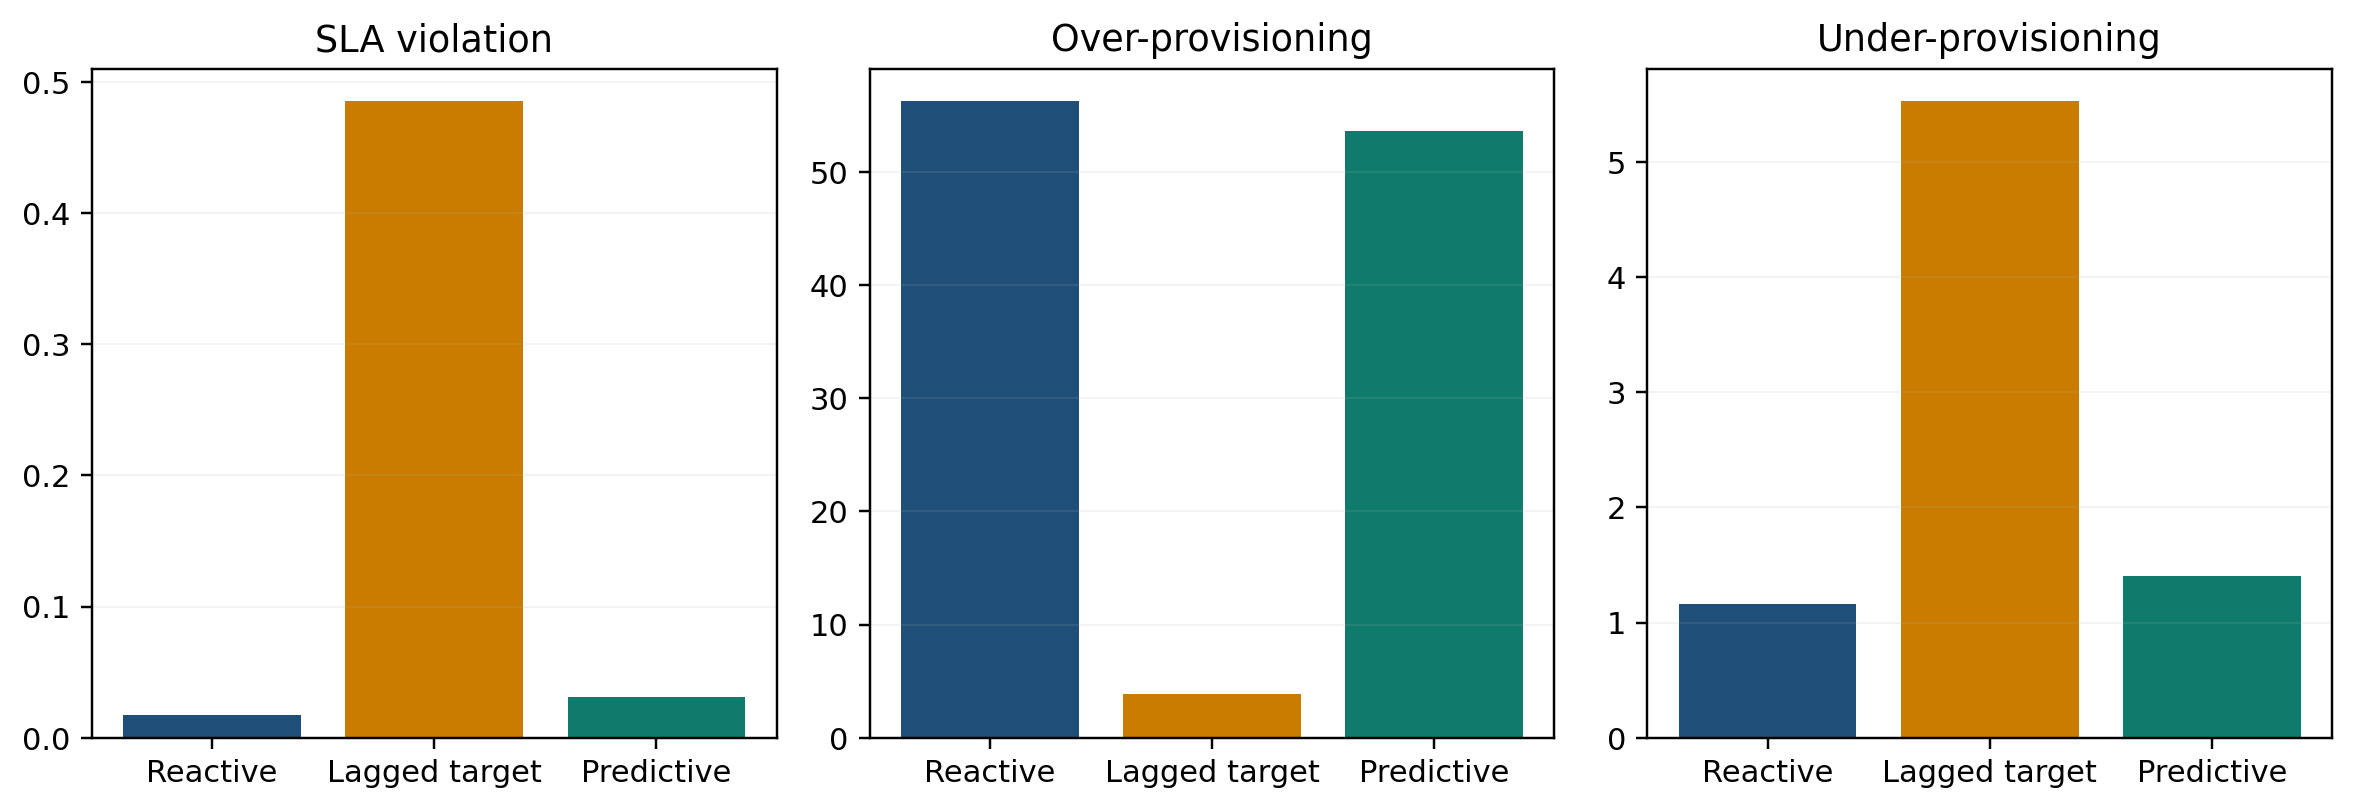
\includegraphics[width=\linewidth]{../experiments/results/service_cohort_broad/figures/service_policy_summary.png}
  \caption{Service-level policy summary across the audited 139-service cohort. The lagged baseline exposes the naive target-chasing extreme, while the predictive controller no longer preserves the earlier service-level action-reduction headline under broader coverage.}
  \label{fig:service-policy-summary}
\end{figure}

\subsection{Trace-driven control comparison}

The aggregate control comparison is driven by a trained uncertainty-aware forecaster rather than by a placeholder forecast source. Table~\ref{tab:policy-results} now summarizes three policies. The reactive threshold policy achieves almost zero SLA violation, but only by carrying a very conservative mean capacity of 0.821 against an average required capacity of 0.470. The lagged target-tracking baseline occupies the opposite extreme: it nearly eliminates over-provisioning (0.013) and keeps mean reserved capacity close to the required load (0.469), but it incurs 47.1\% SLA violation and 1616 scaling actions because one-step-lagged target chasing is too unstable. The predictive policy sits between these extremes. It raises SLA violation to 3.46\%, but cuts over-provisioning by 59.8\% relative to reactive control and keeps mean reserved capacity at 0.610. This is a meaningful systems trade-off rather than an artifact of incomparable units, because all three policies are evaluated in the same normalized required-capacity space and the predictive route applies the same headroom logic to both forecasts and realized demand.

\begin{table}[htbp]
  \centering
  \caption{Reactive, lagged-target, and predictive capacity control on the 5-minute evaluation horizon.}
  \label{tab:policy-results}
  \scriptsize
  \setlength{\tabcolsep}{1.5pt}
  \renewcommand{\arraystretch}{0.96}
  \begin{tabular}{lccccc}
    \toprule
    Policy & SLA & Over & Under & Acts & Cap. \\
    \midrule
    Reactive threshold & 0.001 & 0.351 & 0.000 & 43 & 0.821 \\
    Lagged target tracking & 0.471 & 0.013 & 0.014 & 1616 & 0.469 \\
    Predictive & 0.035 & 0.141 & 0.001 & 589 & 0.610 \\
    \bottomrule
  \end{tabular}
\end{table}

\begin{figure}[htbp]
  \centering
  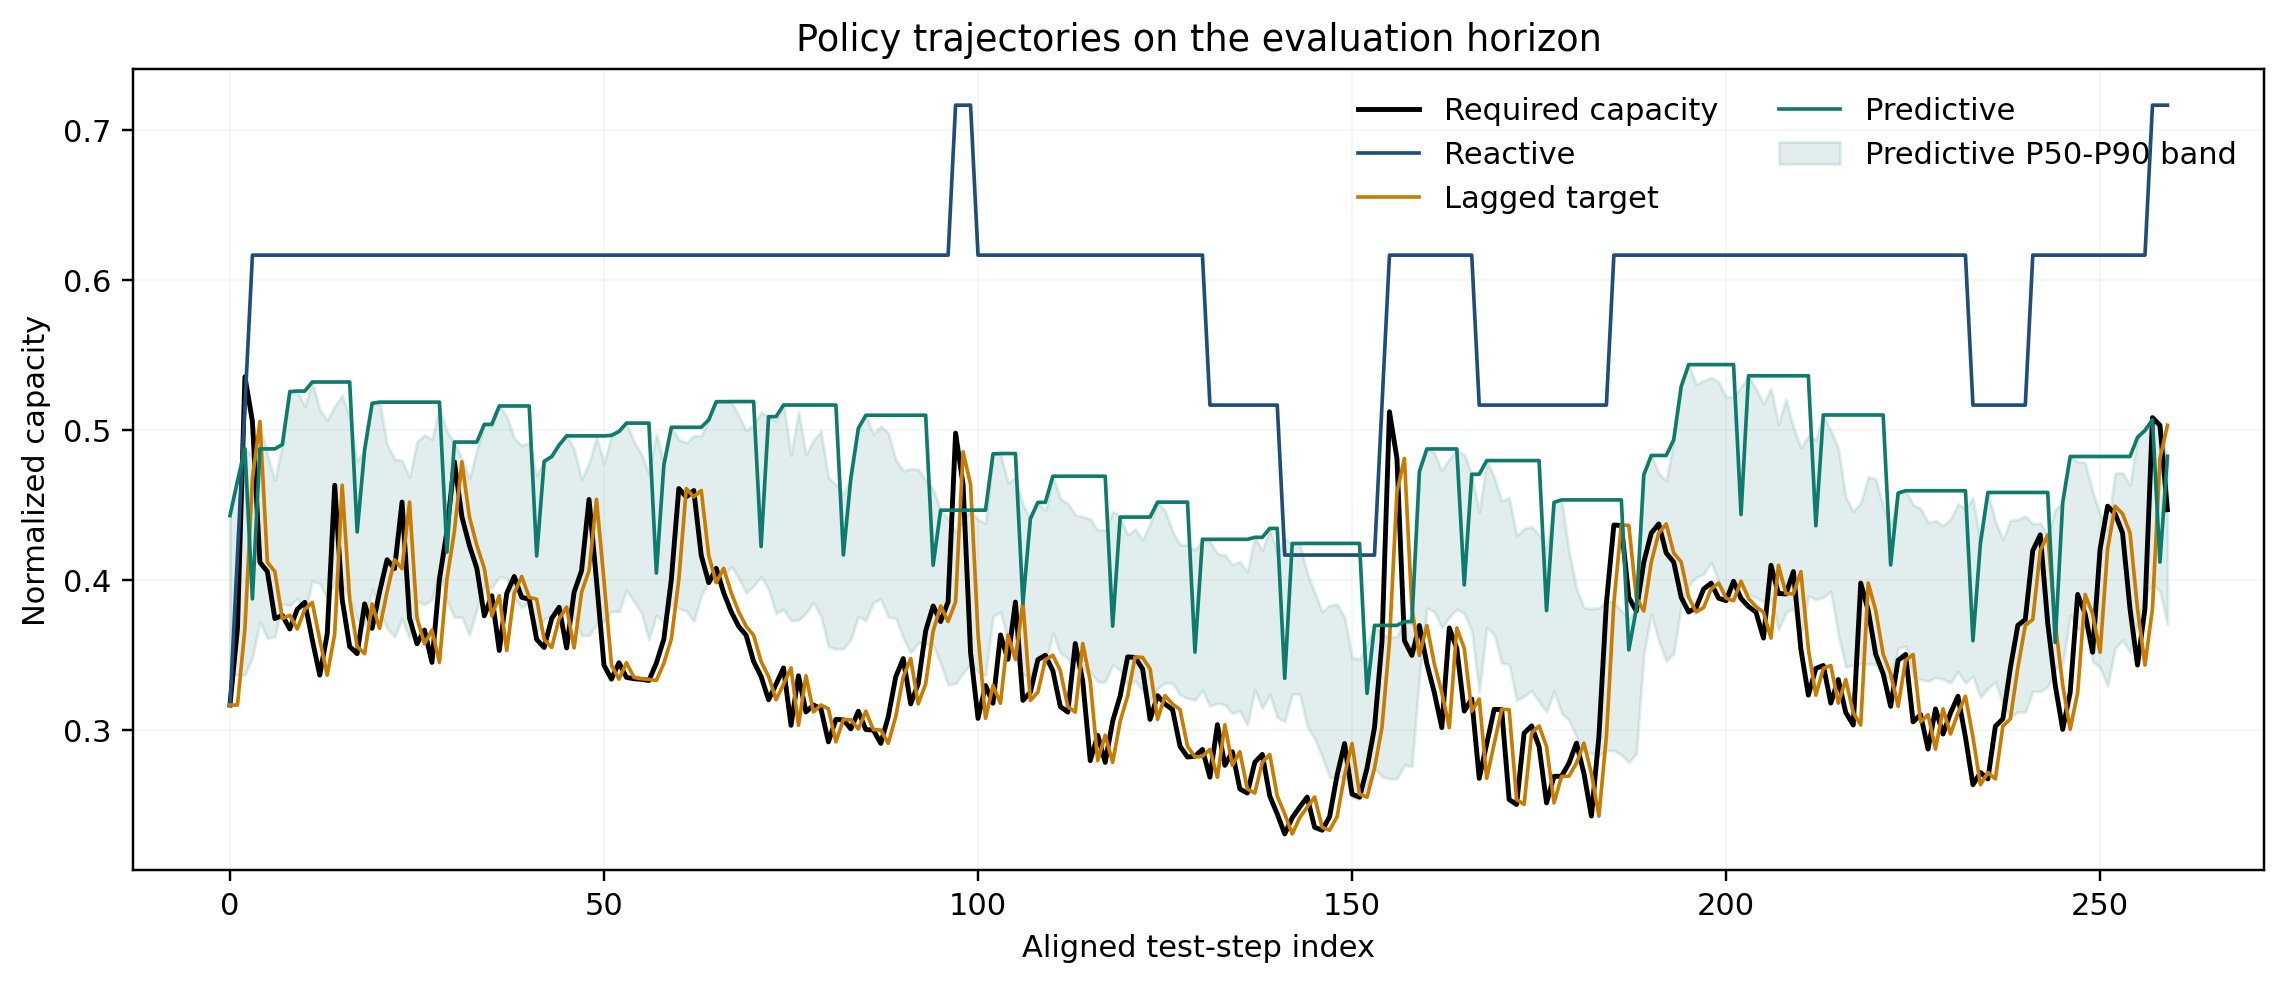
\includegraphics[width=\linewidth]{../experiments/results/figures/policy_capacity_comparison.png}
  \caption{Reactive, lagged-target, and predictive capacity trajectories on the 5-minute evaluation horizon. The lagged baseline shows the failure mode of naive target chasing, while the predictive policy follows the calibrated high-quantile forecast with far lower SLA risk.}
  \label{fig:policy-capacity}
\end{figure}

\subsection{Policy ablation and sensitivity}

The control analysis is now deeper than a single reactive-versus-predictive table. Table~\ref{tab:policy-ablation} shows that the current controller depends heavily on two ingredients: a conservative scale-out margin and cooldown-controlled scale-in. Removing the scale-out margin raises SLA violation from 0.0346 to 0.1137. Removing cooldown keeps over-provisioning relatively low, but pushes the action count from 589 to 1617 and also raises SLA violation to 0.1119. A median-only policy is clearly unacceptable in this setup, with SLA violation rising to 0.3337. By contrast, removing the scale-in guard has almost no effect, which suggests that the current aggregate trace is dominated by scale-out uncertainty rather than scale-in ambiguity.

\begin{table}[htbp]
  \centering
  \caption{Predictive-policy ablation on the 5-minute evaluation route.}
  \label{tab:policy-ablation}
  \scriptsize
  \setlength{\tabcolsep}{1.5pt}
  \begin{tabular}{p{1.65cm}ccccc}
    \toprule
    Variant & SLA & Over & Under & Acts & Cap. \\
    \midrule
    Full predictive policy & 0.035 & 0.141 & 0.001 & 589 & 0.610 \\
    No scale-out margin & 0.114 & 0.089 & 0.004 & 589 & 0.555 \\
    No cooldown & 0.112 & 0.100 & 0.005 & 1617 & 0.565 \\
    Median only & 0.334 & 0.035 & 0.017 & 359 & 0.488 \\
    No scale-in guard & 0.035 & 0.141 & 0.001 & 589 & 0.610 \\
    \bottomrule
  \end{tabular}
\end{table}

Figure~\ref{fig:policy-pareto} extends the same argument with a sweep over scale-out margin and cooldown settings. The chosen default point $(m=0.10, c=8)$ is not globally optimal on any single axis, but it sits near the middle of the observed Pareto surface. Smaller margins reduce over-provisioning but push SLA risk sharply upward, while larger margins and longer cooldown improve SLA protection by consuming more steady capacity. This is exactly the kind of operational trade-off that a systems paper should make explicit rather than hide behind a single best configuration.

\begin{figure}[htbp]
  \centering
  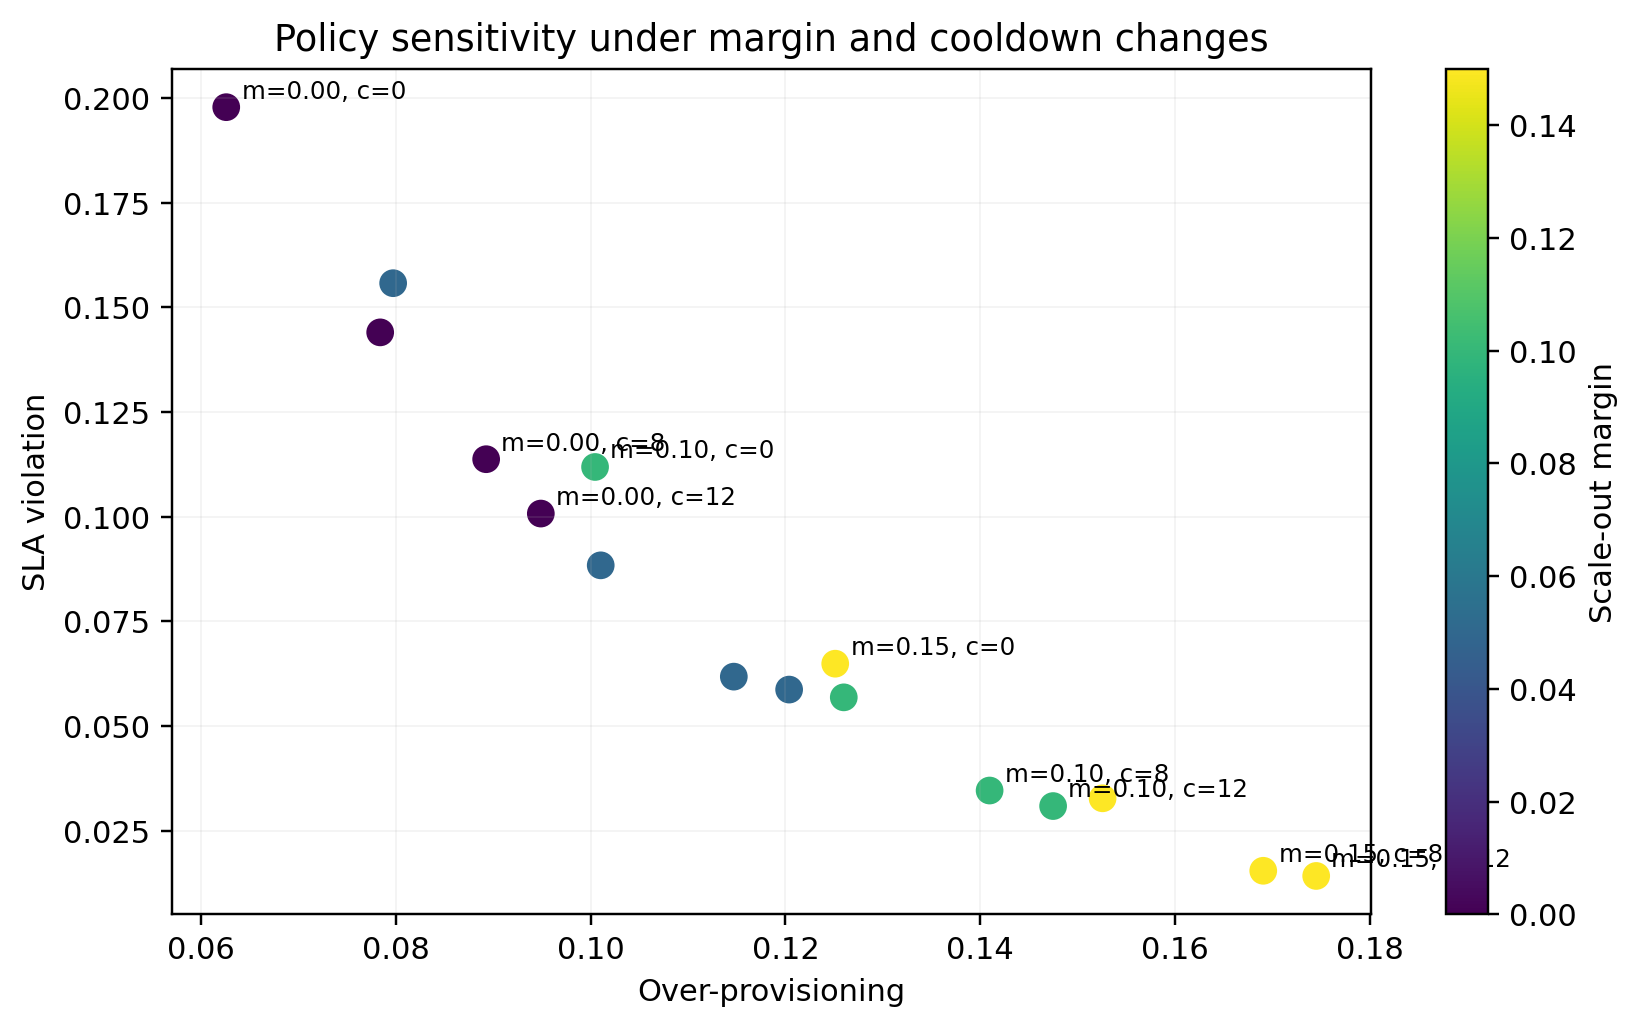
\includegraphics[width=0.82\linewidth]{../experiments/results/figures/policy_pareto_sensitivity.png}
  \caption{Sensitivity of the predictive controller to scale-out margin and cooldown. The selected default operates in the middle of the observed SLA-versus-over-provisioning trade-off.}
  \label{fig:policy-pareto}
\end{figure}

The boundary is now narrower. A public trace-driven simulator with a trained forecasting backbone, calibration evidence, and policy ablations is strong evidence for reproducible control trends, but it is still not a substitute for a live production deployment. The current result should therefore be interpreted as trace-level evidence about when predictive control succeeds and when it fails, not as proof that the same policy would transfer unchanged to a real cluster controller.
